\documentclass[12pt, a4paper]{article}
\usepackage[utf8]{inputenc}
\usepackage{geometry}
\geometry{margin=1in}
\usepackage{graphicx}
\usepackage{booktabs}
\usepackage{amsmath}
\usepackage[round]{natbib}
\usepackage[hidelinks]{hyperref}
\usepackage{float}
\linespread{1.25}

\title{\textbf{Report 1: Preliminary Analysis of Noun Memorability\\
and Syntactic Structure in Sentence Recognition}}
\author{Shreyas Deb, Yajat Lakhanpal, Prasoon Dev}

\begin{document}

\maketitle

% ─────────────────────────────────────────────────────────────
\section{Introduction and Background}
% ─────────────────────────────────────────────────────────────

Early transformational accounts of sentence memory — critically examined by
both \citet{bregman1968} and \citet{james1973} — held that speakers encode
sentences by reducing them to a canonical ``kernel'': a simple, active,
affirmative, declarative form, supplemented by syntactic tags indicating the
transformations required to restore the original surface structure. Under this
\textit{kernel-plus-tag} model, the passive voice, negation, and interrogative
form are each stored as single, independently forgettable memory-trace
components. A clear empirical consequence follows: if syntactic features are
genuinely independent and all-or-none, then a participant who fails to identify
the correct syntactic form on a first attempt should perform at chance on a
second attempt, because the relevant trace component would simply be absent
\citep{bregman1968}.

\citet{bregman1968} tested this prediction directly. They presented 20 five-word
sentences — each instantiated in active, passive, negative, and question forms —
to 60 undergraduates in a forced-choice recognition procedure. After participants
committed to a first-guess syntactic label, Bregman and Strasberg examined
whether second guesses on errors still carried information. If syntactic features
were all-or-none traces, they should not. Instead, second-guess accuracy was
reliably above chance across both replications (\(\chi^2(4) = 20.8,\ p < .001\)).
A shift analysis revealed a consistent \textit{active--passive subcategory}:
participants who confused active with passive sentences did so systematically,
while negative and question confusions arose largely as a forced-choice artefact.
Post-experimental interview data confirmed that participants reconstructed the
active--passive distinction from retained semantic information — action imagery,
truth value, affective response, and noun salience — rather than from any stored
syntactic symbol \citep{bregman1968}. Bregman and Strasberg therefore concluded
that once a sentence has been comprehended, the properties of the transmission
code need not be preserved in the memory trace; what enters long-term memory
refers to the \textit{semantic} properties of the message, not the surface form
in which the message was delivered.

This conclusion carries a specific implication: the semantic substance retained
from a sentence — its ``gist'' — should be largely decoupled from its verbatim
wording. \citet{begg1971} examined this dissociation directly in a continuous
recognition paradigm. Using two parallel lists of 502 sentences drawn from
novels and rated for imagery, Begg tested eight participants on meaning judgments
(``Have you seen a sentence with this meaning before?'') and wording judgments
(``Are these the exact words you saw?'') across lags of 2 to 64 intervening
sentences. Meaning recognition declined monotonically and substantially with lag
(\(r = -.996,\ p < .001\)), whereas wording recognition was entirely uncorrelated
with lag (\(r = -.107\), \textit{n.s.}) and remained above chance at approximately
0.62 correct, a level consistent with wording memory relying on reconstruction
rather than on an intact trace. Furthermore, meaning and wording judgments
were stochastically independent: the probability of a jointly correct judgment
approximated the product of the marginal probabilities
(\(P_{cM} \cdot P_{cW} = .778\) vs.\ observed \(P_{cM\&W} = .790\)),
indicating that the two systems draw on distinct memory representations
\citep{begg1971}. Begg interpreted these findings as support for a dual-trace
model in which concrete sentence meaning is stored as a nonverbal spatial image
while specific words are reconstructed from that image at retrieval rather than
preserved as a sequential verbal string. Crucially, meaning recognition was no
less accurate for paraphrase probes than for identical-wording probes, confirming
that syntactic and lexical cues provide no facilitation when retrieving the stored
meaning image \citep{begg1971}.

If both syntactic tags and verbatim word sequences are unreliably retained, the
question shifts to what drives the reconstructive process when the gist image is
retrieved. \citet{james1973} identified two systematic biases. First, spontaneous
speech production favours active constructions; because recall is itself a
constructive act governed by the same production preferences, participants
disproportionately reconstruct passive sentences as active. Second, and more
directly relevant to the present study, speakers tend to initiate a recalled
sentence with the most salient noun in the stored semantic representation —
operationalised as imagery value \textit{(I-value)} — regardless of whether that
noun originally occupied the surface subject or object position. James and
colleagues instantiated this manipulation in a 4 (noun imageability: HH, HL,
LH, LL) $\times$ 2 (voice: active, passive) free-recall design, selecting
high-imageability nouns (ratings $> 5.90$) and low-imageability nouns
(ratings $< 3.50$) on a 7-point scale. The voice-error probability data
\citep[Table~2]{james1973} were highest for LH sentences (0.245 active;
0.333 passive) and lowest for HL sentences (0.029 active; 0.049 passive),
with HH and LL at intermediate and approximately equal rates — precisely the
pattern predicted by a reconstructive account in which the high-imageability
noun captures the sentence's ``theme'' and is preferentially placed in subject
position at recall \citep{james1973}. This ordering was inconsistent with all
five storage hypotheses evaluated — including the kernel-plus-tag model — without
supplementary reconstructive assumptions. Overall sentence recall also scaled
monotonically with imagery load: HH $>$ HL $\approx$ LH $>$ LL
\citep[Table~1]{james1973}.

Taken together, these three lines of work converge on a framework in which
sentence memory is driven primarily by the semantic and imagistic properties of
constituent words, while verbatim syntactic form occupies a secondary,
independently stored representation that decays more rapidly and is
reconstructed rather than retrieved. The present experiment builds directly on
this framework by adapting the noun-imageability manipulation of
\citet{james1973} to a \textit{recognition} rather than recall paradigm, using
a continuous presentation procedure modelled on \citet{begg1971}. Whereas James
and colleagues measured voice-error probability in free recall, we assess
\textit{corrected} hit rates for sentence meaning recognition (Immediate
Recognition, IR) and separately measure participants' ability to discriminate
the grammatical voice of the encoded sentence (Wording Recognition, WR). This
dual-response design mirrors Begg's separation of meaning and wording judgments,
enabling us to test whether noun imageability selectively affects semantic gist
encoding (IR), surface-form retention (WR), or both. If the reconstructive
framework is correct, imageability should affect IR — because the richness of the
image trace governs whether gist is recognised upon second presentation — while
WR should remain largely insensitive to noun imageability but may show a
directional advantage for active over passive voice, consistent with the
production bias documented by \citet{james1973}.


% ─────────────────────────────────────────────────────────────
\section{Methods}
% ─────────────────────────────────────────────────────────────

\subsection{Experimental Design and Stimuli}

This study employed a $4 \times 2$ fully within-participants design, with Noun
Condition (HH, HL, LH, LL) and Grammatical Voice (Active, Passive) as the two
factors. Simple Subject-Verb-Object (S-V-O) sentences were generated by
systematically varying the imageability of the subject and object nouns. High-
and low-imageability nouns were drawn from established word imageability norms
following the same operationalisation used by \citet{james1973}, while verbs
were selected from a fixed set of medium-concreteness action verbs to minimise
variability across conditions. Automated fluency checks and semantic-coherence
filters removed ungrammatical or implausible sentences, followed by manual
screening.

This procedure yielded four noun conditions:
\begin{itemize}
    \item \textbf{HH:} High-imageability subject, High-imageability object.
    \item \textbf{HL:} High-imageability subject, Low-imageability object.
    \item \textbf{LH:} Low-imageability subject, High-imageability object.
    \item \textbf{LL:} Low-imageability subject, Low-imageability object.
\end{itemize}

From the resulting pool, 200 active-voice sentences were selected (50 per noun
condition). Each sentence was then converted into a passive-voice equivalent,
producing paired active and passive variants. This resulted in 400 target
sentences across eight experimental conditions (4 noun conditions $\times$ 2
voices). Sentences were kept short ($\leq 8$ words) and excluded proper nouns
to inhibit extraneous mnemonic associations. An additional set of high-frequency
filler sentences (prefix \texttt{HF}) was interwoven throughout the stream to
provide false alarm opportunities and mitigate list-learning effects, following
the continuous recognition approach of \citet{begg1971}.

\subsection{Participants and Procedure}

A priori power analysis indicated that 334 valid participants would be required
to achieve adequate statistical power for detecting interaction effects of the
anticipated magnitude. Ultimately, 114 online participants began the experiment,
providing a preliminary dataset.

Participants completed a continuous recognition task comprising three blocks
separated by rest phases to limit fatigue. Each participant was exposed to 48
target sentences (16 per block), balanced across the 8 experimental conditions.
Each target sentence appeared twice: once as an \textit{encoding} trial (first
presentation) and once as a \textit{probe} trial (second presentation, the
recognition test). Stimulus IDs encoded experimental conditions: the prefix
denoted noun condition (\texttt{HH}, \texttt{HVL} $\to$ HL, \texttt{LVH} $\to$
LH, \texttt{LVL} $\to$ LL) and the trailing character denoted voice
(\texttt{A} = active, \texttt{P} = passive).

Upon seeing a probe, participants provided two sequential responses:
\begin{enumerate}
    \item \textbf{Immediate Recognition (IR):} Participants pressed the Spacebar
    if they recognised the sentence's meaning as a repeat from earlier in the
    session. This corresponds to Begg's (\citeyear{begg1971}) meaning judgment.
    \item \textbf{Wording Recognition (WR):} Immediately following an IR press,
    participants made a forced-choice ``Yes/No'' judgment as to whether the probe
    matched the exact grammatical voice (active vs.\ passive) of its initial
    presentation. This corresponds to Begg's (\citeyear{begg1971}) wording
    judgment.
\end{enumerate}

\subsection{Data Cleaning and Exclusion Criteria}

Raw event logs were processed through a dedicated R pipeline. Practice-phase
rows, inter-stimulus gap-time metadata events, and rest-phase markers were
removed. A sequential \texttt{block\_id} (1--3) was assigned per participant
based on rest-phase boundaries.

An objective block-level validity criterion was applied, based on performance
on embedded validation sentences. Three event types were used:
\textit{correct validation} (IR pressed on a validation repeat),
\textit{wrong IR press} (IR pressed on a non-repeat sentence), and
\textit{missed validation} (no IR press on a validation repeat). A block was
retained only if:
$$
\text{Correct Validations} > \frac{\text{Wrong IR Presses}}{2} + \text{Missed Validations}
$$
Blocks failing this criterion were excluded from all downstream analyses. This
block-level filter retained 329 of a possible 336 participant-blocks
(112 of 114 participants; 97.9\% pass rate). Block-level participant counts
after exclusion were: Block 1 ($n = 108$), Block 2 ($n = 109$), Block 3
($n = 112$).

\subsection{Computed Measures and Analytical Approach}

\paragraph{IR Corrected Recognition.}
To isolate discrimination sensitivity from individual response bias, the primary
outcome was the corrected recognition score:
$$
\text{Corrected IR} = \text{Hit Rate} - \text{False Alarm (FA) Rate}
$$
\textit{Hit rate} was calculated per participant per noun condition (collapsed
across voice for the primary Kruskal-Wallis test; by condition $\times$ voice
for the 8-cell analyses): the proportion of target probe trials on which the
participant pressed the Spacebar. Missed probes counted as 0. \textit{False alarm
rate} was calculated globally per participant as the proportion of HF-filler
first showings that received an erroneous IR press; validation sentences were
excluded from the FA denominator because they serve a different experimental
function. The global FA rate was then subtracted uniformly from all
condition-level hit rates for that participant. This approach isolates true
discrimination from the liberal-versus-conservative response bias documented
in Figure~\ref{fig:hit_fa}, paralleling signal-detection corrections while
avoiding the normality assumption required by $d'$, which is inappropriate
for the bounded $[-1, 1]$ range of these scores.

\paragraph{WR Accuracy.}
For each target probe on which an IR press was made, a wording judgment was
recorded (\texttt{wr\_accuracy = 1} correct; 0 incorrect). WR accuracy was
computed as the proportion of correct wording judgments per participant per
condition, mirroring the wording judgment measure in \citet{begg1971}.

\paragraph{IR Reaction Time.}
Reaction time (RT) was extracted from the \texttt{ir\_reaction\_time\_ms} column
on IR-pressed events for target probes. Implausible RTs ($> 10{,}000$ ms) were
excluded.

\paragraph{Statistical Tests.}
All analyses aggregated scores to the participant level first, to avoid
pseudoreplication. Differences across the four noun conditions were assessed
with Kruskal-Wallis tests, chosen because bounded accuracy scores violate the
normality assumptions of parametric ANOVA. Effect size was quantified using
$\varepsilon^2 = (H - k + 1)/(n - k)$, where $H$ is the Kruskal-Wallis
statistic, $k$ is the number of groups, and $n$ is the number of participants.
Significant omnibus tests were followed by pairwise Wilcoxon rank-sum tests
with Holm--Bonferroni correction. Voice effects (Active vs.\ Passive) were
assessed with paired Wilcoxon signed-rank tests. Above-chance WR performance
was assessed with one-sample Wilcoxon tests against $\mu = 0.5$. Monotonic
associations were quantified using Spearman's $\rho$. All analyses were
conducted in R (version $\geq 4.3$) using \texttt{dplyr}, \texttt{ggplot2},
\texttt{tidyr}, \texttt{stringr}, and \texttt{scales}. Figures were saved
at 300 DPI.


% ─────────────────────────────────────────────────────────────
\section{Analysis and Results}
% ─────────────────────────────────────────────────────────────

\subsection{Descriptive Overview and Response Bias}

Across the 5,264 valid target probe trials, the overall mean hit rate was $0.832$
and the mean false alarm rate was $0.160$ (range: $0.000$--$0.427$). After
correction, the overall mean corrected IR was $M = 0.673$ ($Mdn = 0.708$,
range: $-0.141$--$1.000$).

As shown in Figure~\ref{fig:hit_fa}, there is a significant positive correlation
between hit rate and false alarm rate at the participant level (Spearman
$\rho = .208$, $p = .028$), confirming that more liberal responders accumulate
both more hits and more false alarms simultaneously. This response bias motivates
the corrected recognition measure as the primary dependent variable. Response
time distributions (Figure~\ref{fig:rt_density}) display the characteristic
right-skewed shape expected for memory retrieval latencies, with the bulk of
responses concentrated between 800 and 2,500 ms.

\begin{figure}[H]
    \centering
    \begin{minipage}{0.48\textwidth}
        \centering
        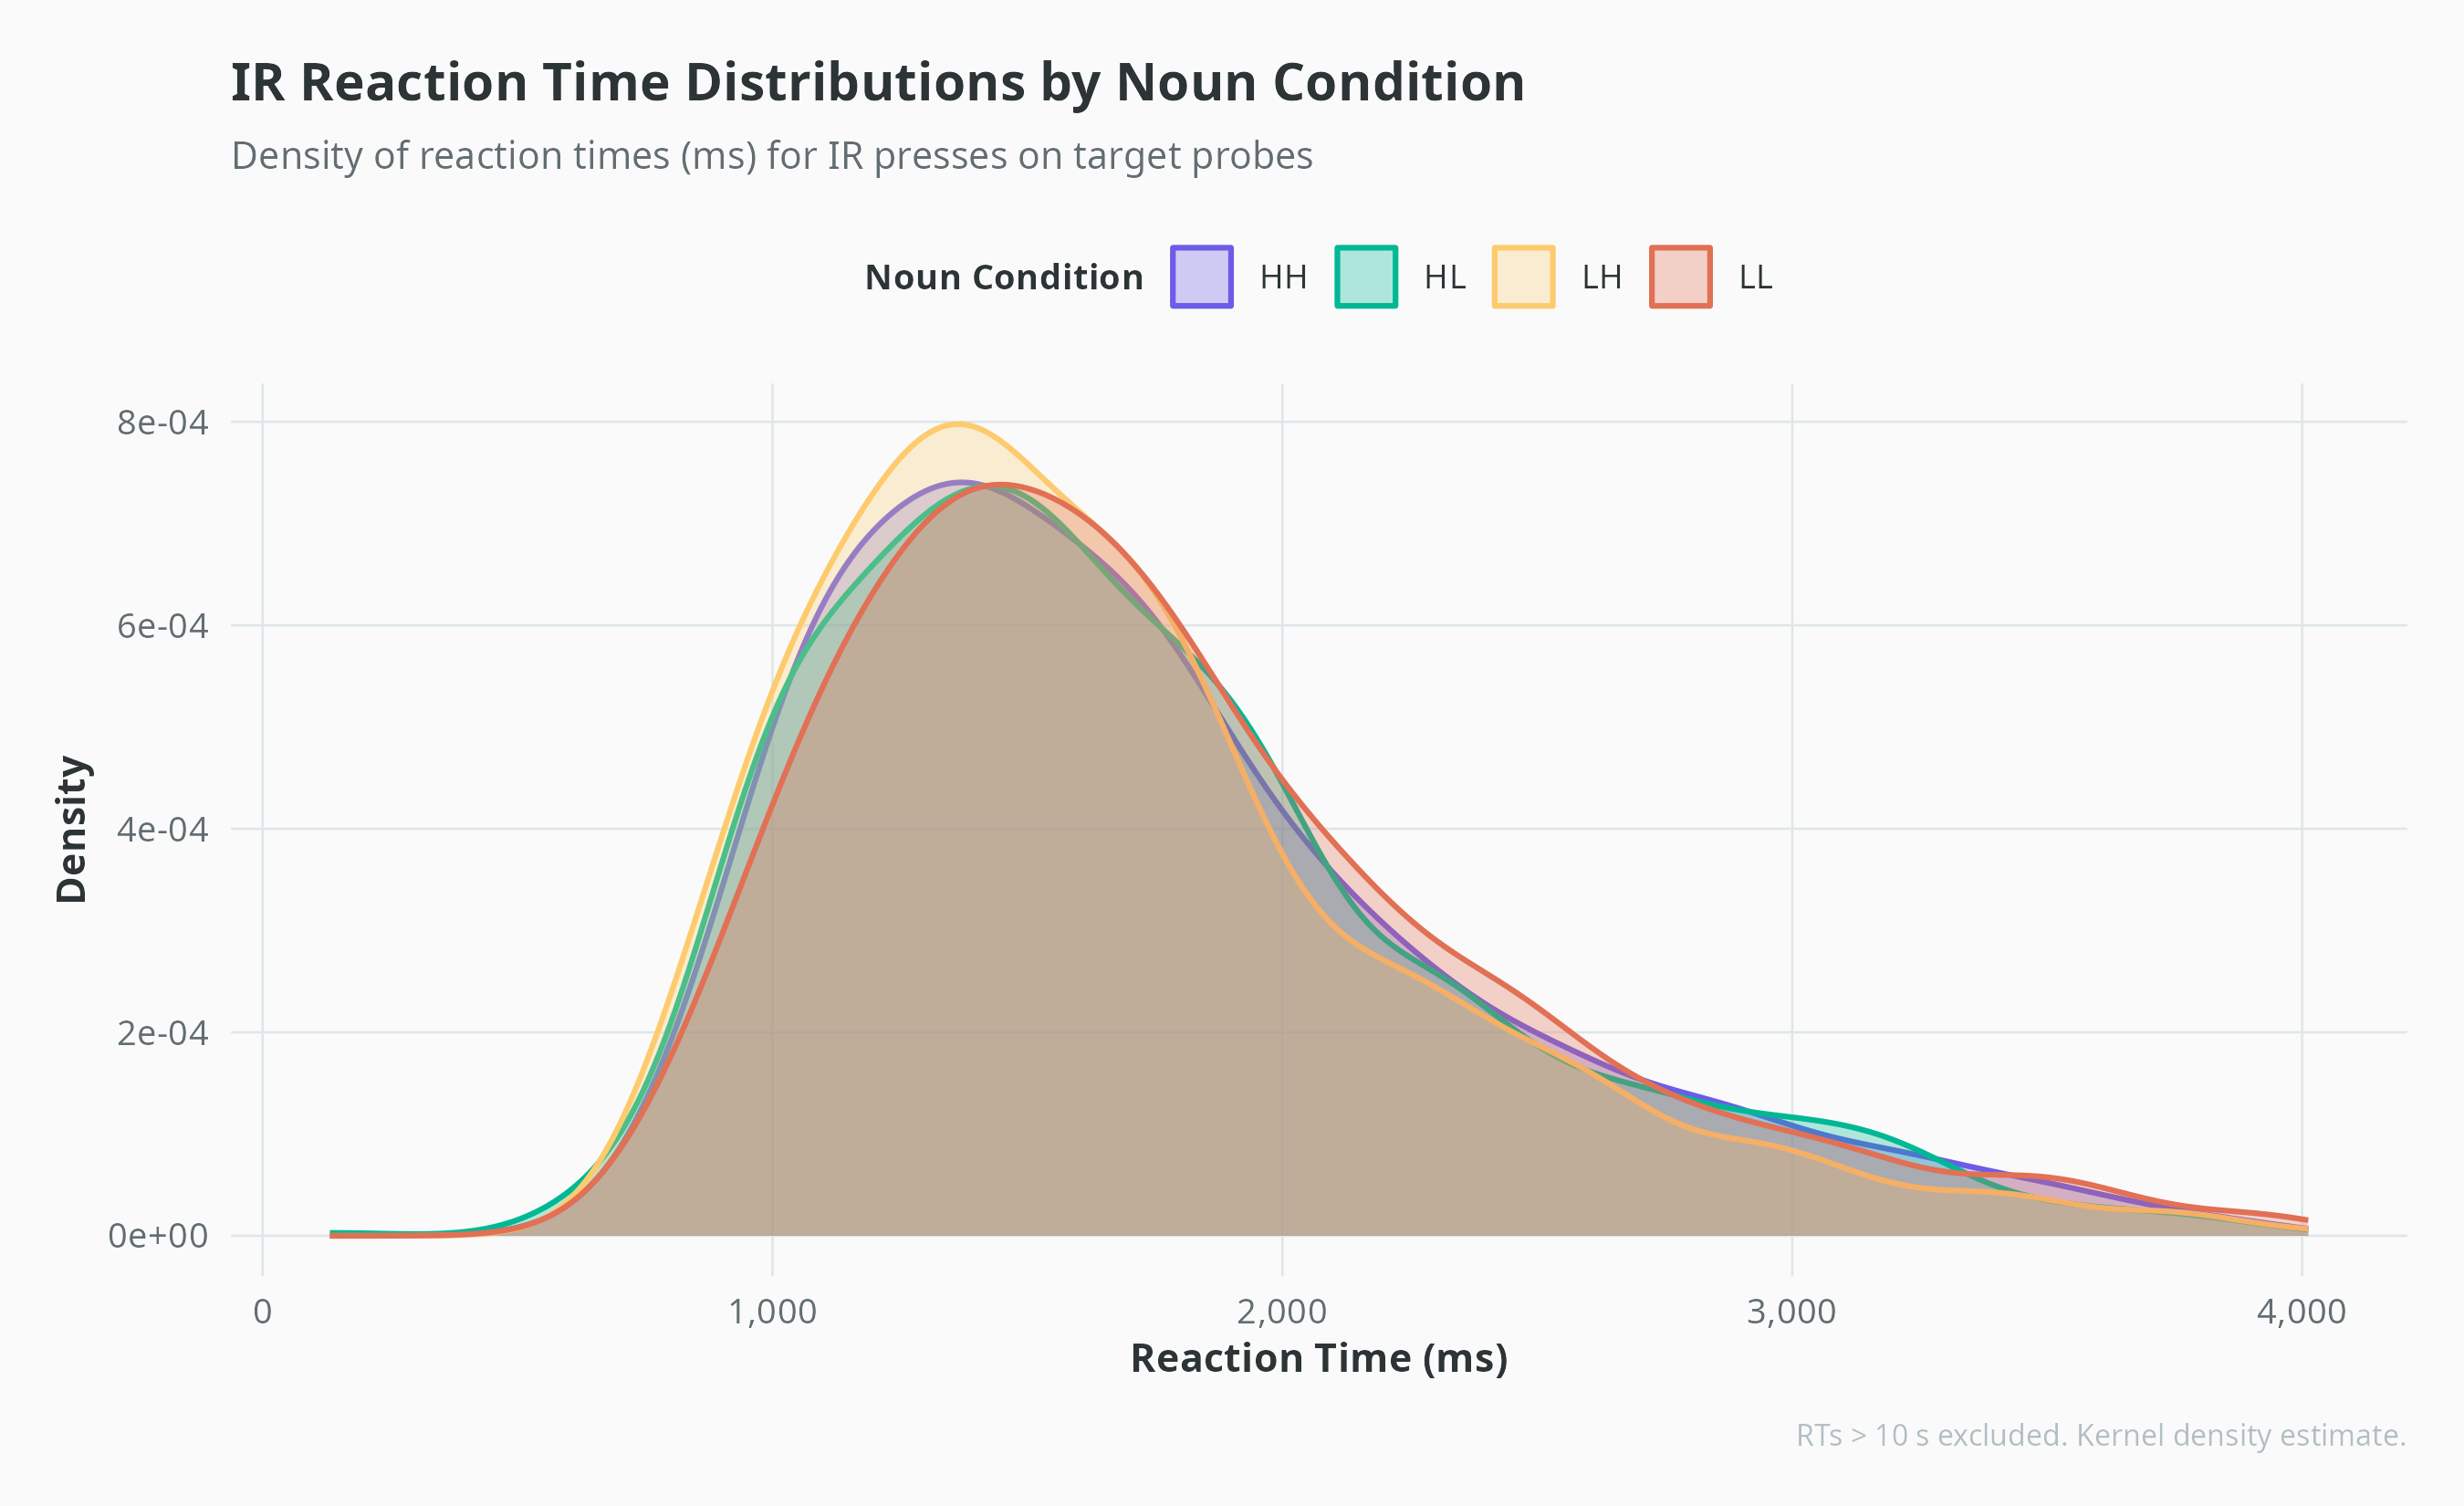
\includegraphics[width=\linewidth]{../../plots/05_ir_rt_density.png}
        \caption{Density distributions of Immediate Recognition reaction times
        (ms) by noun condition. All four conditions show the characteristic
        right-skewed latency profile of memory retrieval; RTs $> 10{,}000$ ms
        excluded.}
        \label{fig:rt_density}
    \end{minipage}\hfill
    \begin{minipage}{0.48\textwidth}
        \centering
        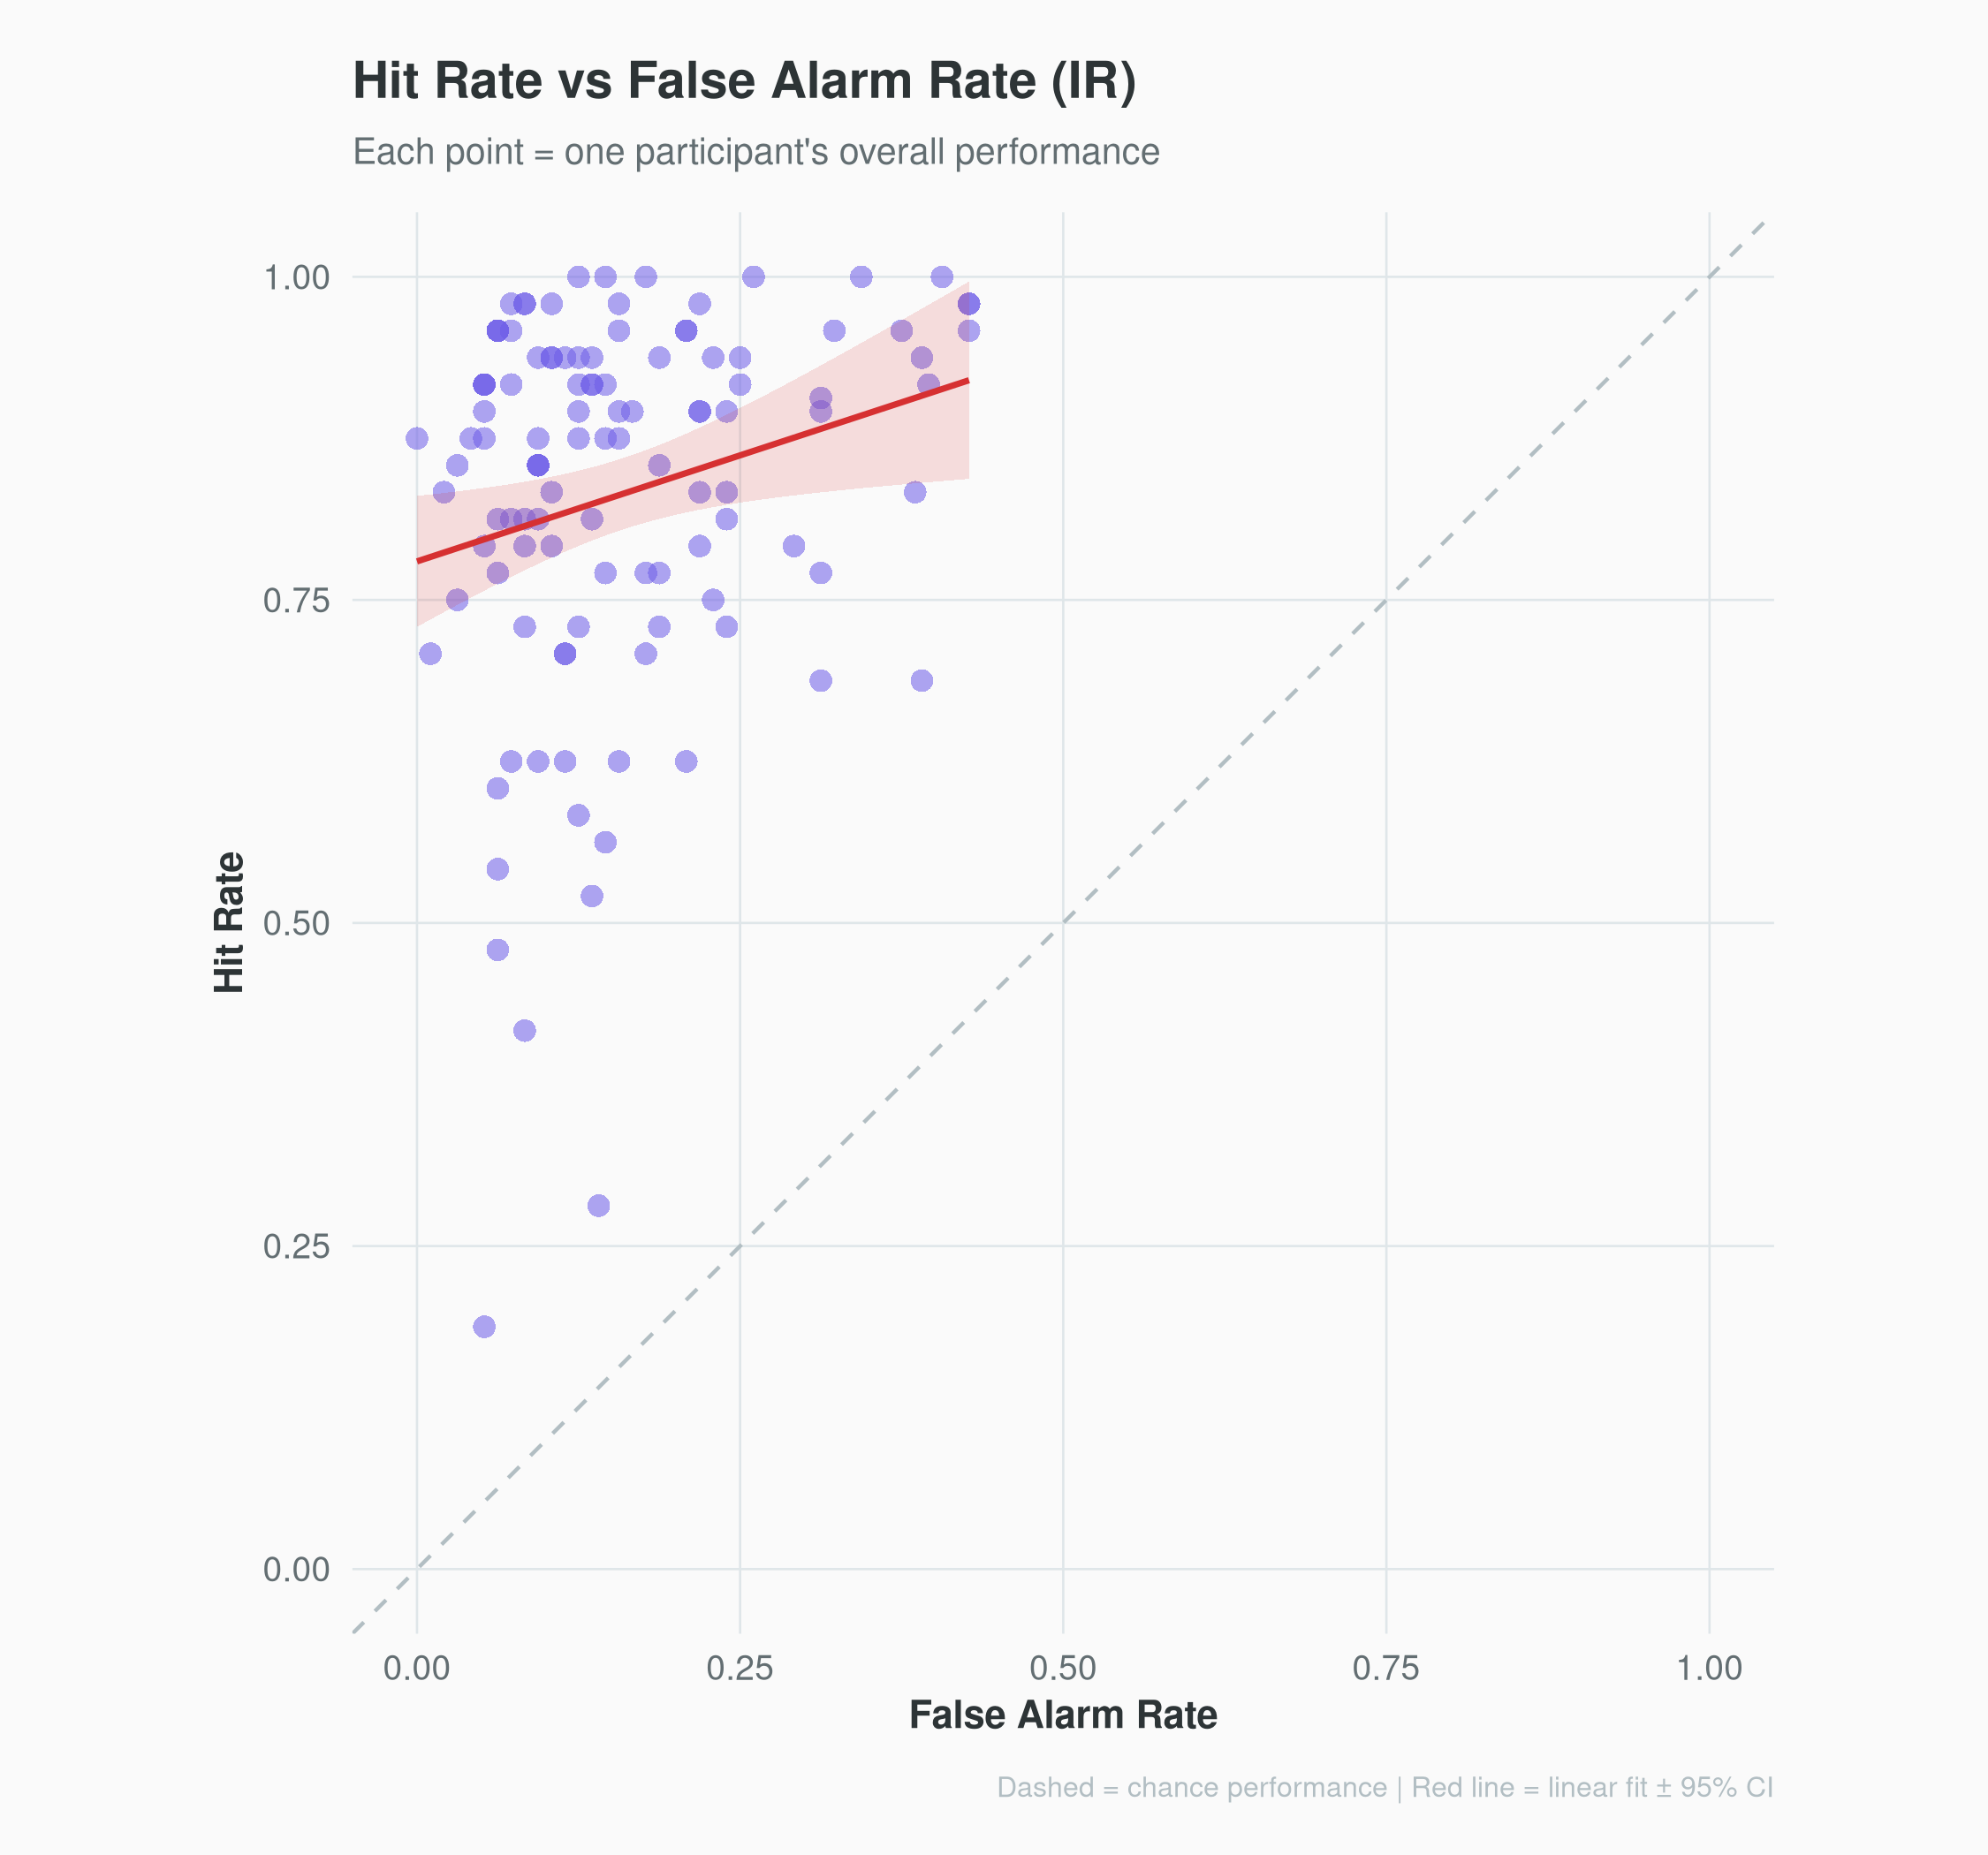
\includegraphics[width=\linewidth]{../../plots/06_hit_vs_fa.png}
        \caption{Per-participant hit rate against false alarm rate. The positive
        linear trend (Spearman $\rho = .208$, $p = .028$) confirms systematic
        response bias, motivating the corrected recognition score. The dashed
        diagonal represents chance ($\text{hit} = \text{FA}$).}
        \label{fig:hit_fa}
    \end{minipage}
\end{figure}

The per-participant heatmap (Figure~\ref{fig:heatmap}) illustrates substantial
between-participant variability in baseline performance. The consistent colour
shift from HH/HL/LH (warmer greens) to LL (cooler reds) within individual rows
confirms that the noun-condition effect is not driven by a small subset of
participants.

\begin{figure}[H]
    \centering
    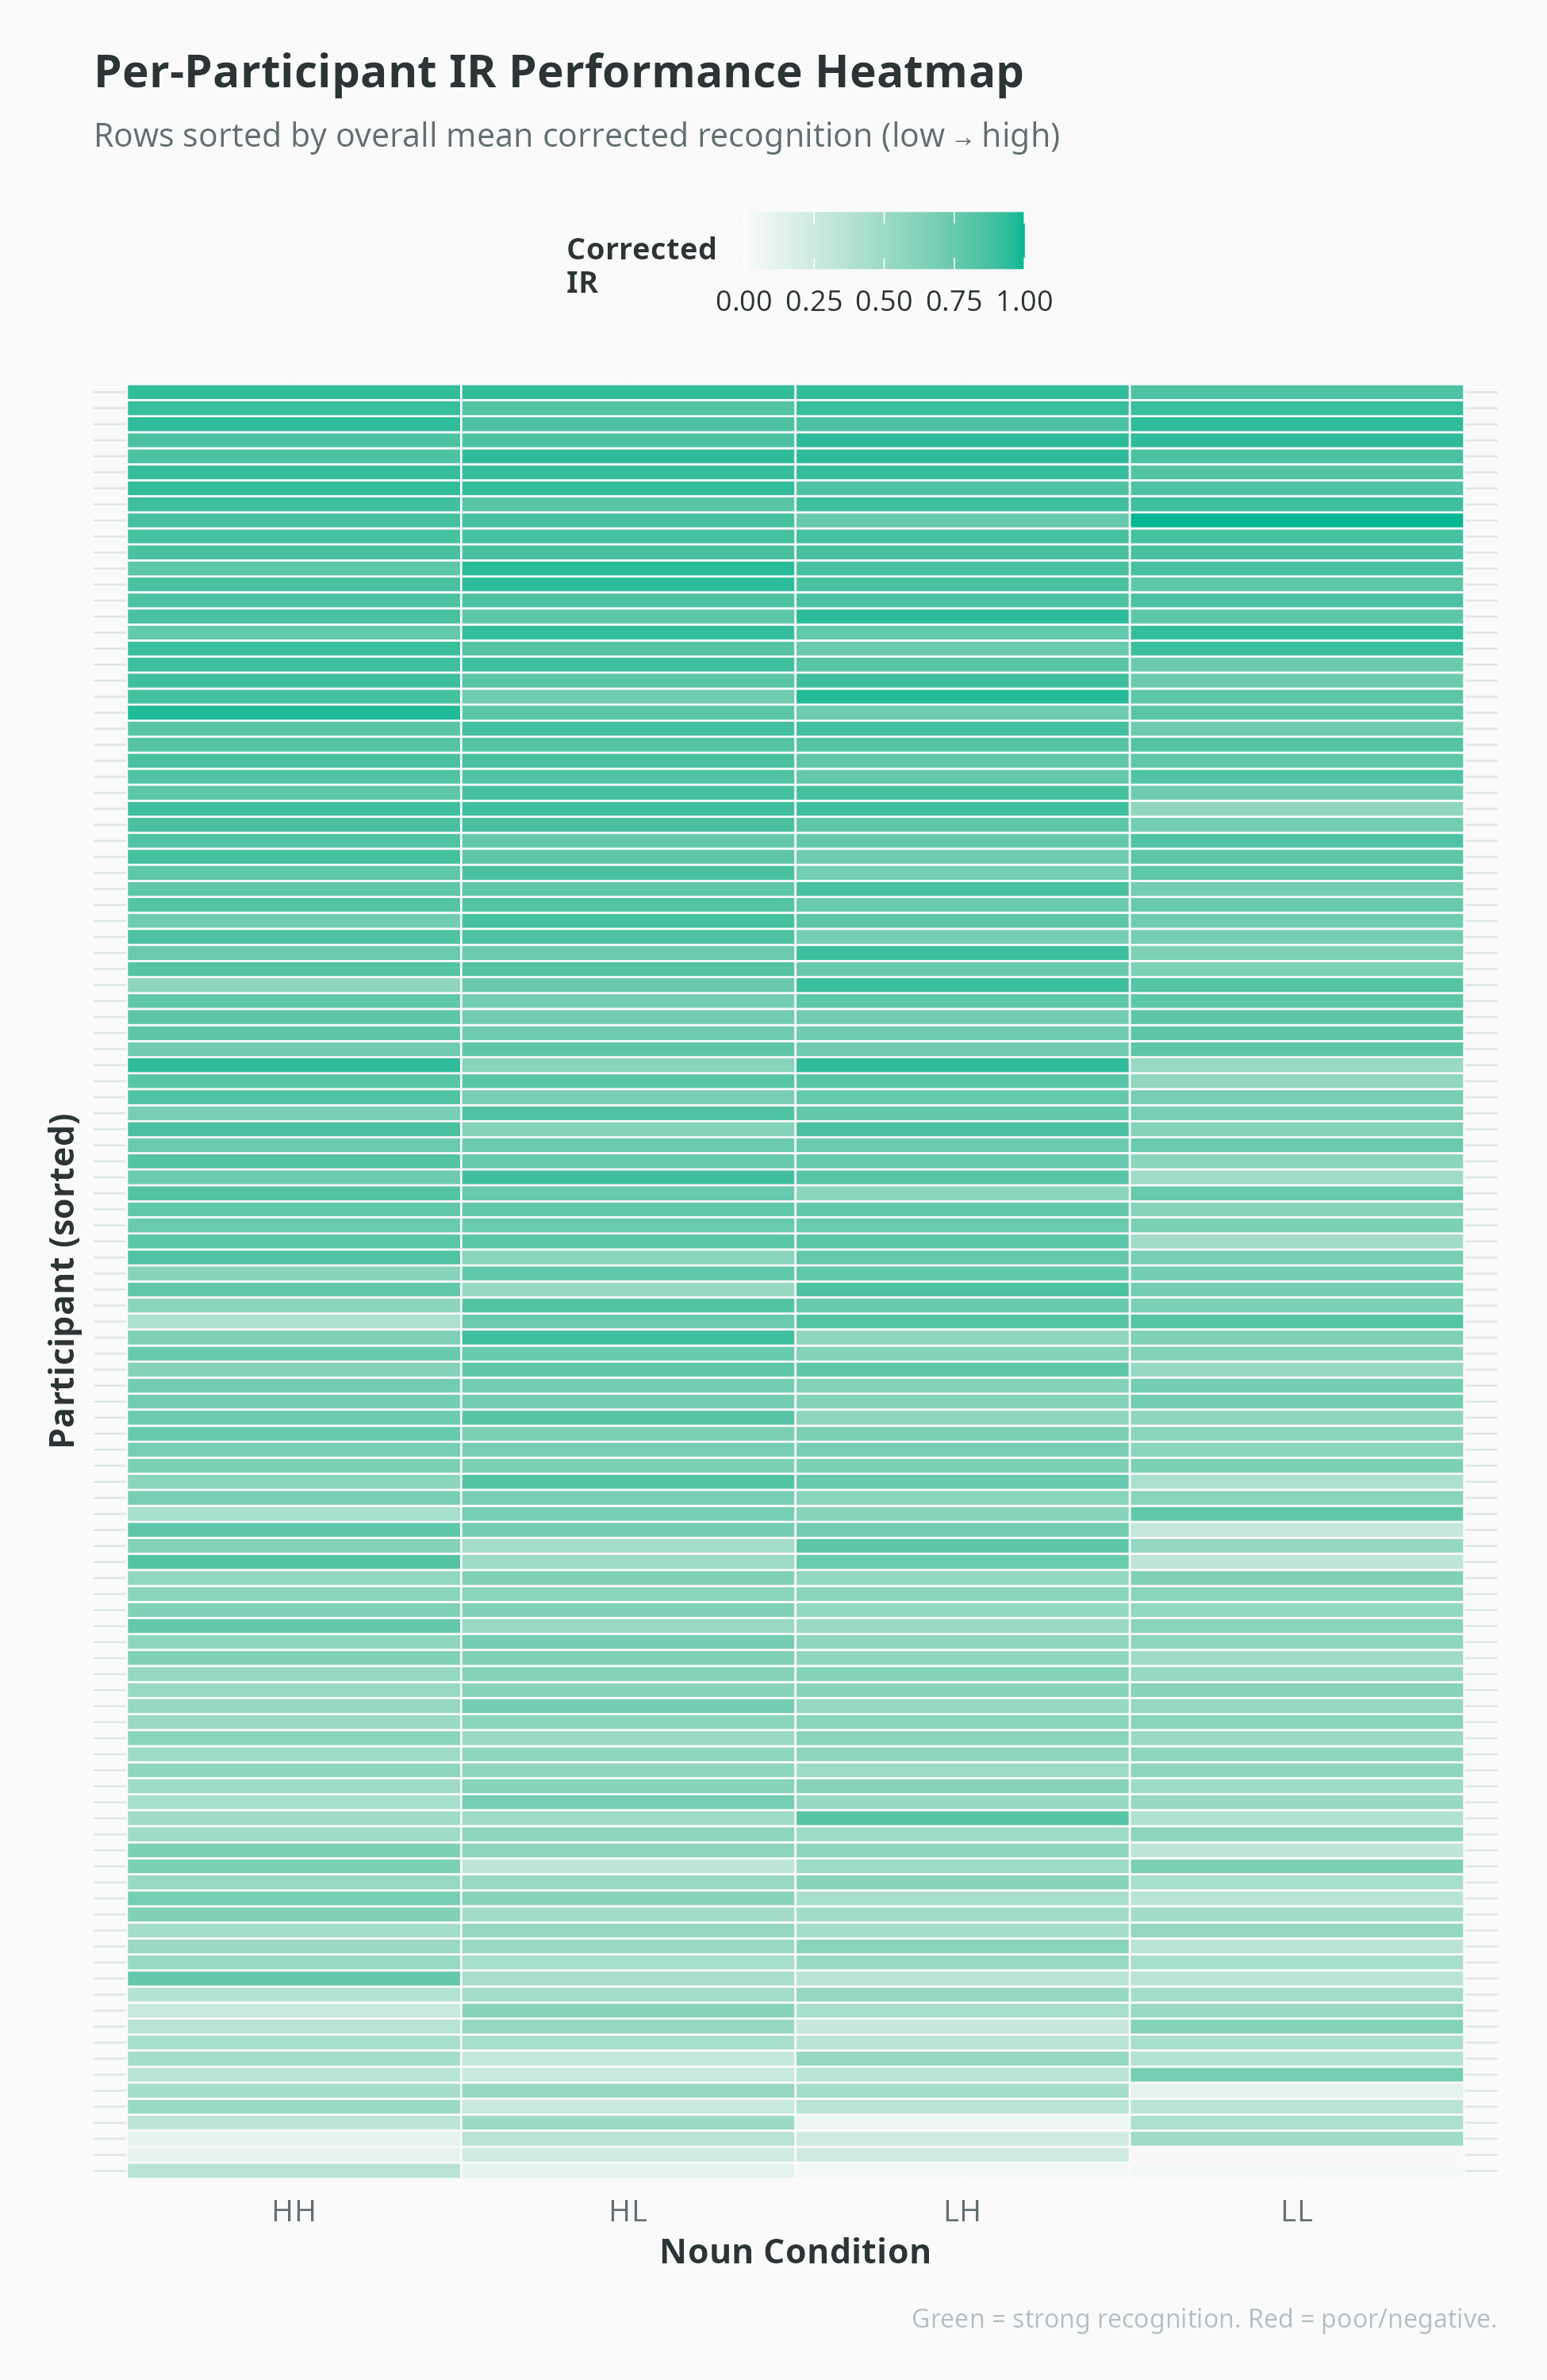
\includegraphics[width=0.7\textwidth]{../../plots/08_participant_heatmap.png}
    \caption{Per-participant corrected IR heatmap. Rows are sorted by overall
    mean corrected recognition (low to high). The rightward shift to cooler
    colours in the LL column is visible within most participants' rows,
    indicating a robust within-subject effect.}
    \label{fig:heatmap}
\end{figure}


\subsection{Main Effect of Noun Condition on Immediate Recognition}

We predicted that noun imageability would positively influence sentence
recognition, following the recall pattern documented by \citet{james1973}.
Table~\ref{tab:ir} summarises corrected IR scores collapsed across grammatical
voice.

\begin{table}[H]
\centering
\caption{Corrected Immediate Recognition (IR) Scores by Noun Condition ($n = 112$)}
\label{tab:ir}
\begin{tabular}{@{}lcccc@{}}
\toprule
Condition & $M$ & $SD$ & $Mdn$ & Range \\ \midrule
HH & 0.689 & 0.185 & 0.740 & $-0.141$ -- $1.000$ \\
HL & 0.691 & 0.177 & 0.708 & $-0.052$ -- $1.000$ \\
LH & 0.679 & 0.188 & 0.729 & $-0.083$ -- $0.979$ \\
LL & 0.632 & 0.189 & 0.656 & $-0.141$ -- $1.000$ \\ \bottomrule
\end{tabular}
\end{table}

A Kruskal-Wallis test revealed a statistically significant main effect of noun
condition on corrected IR, $H(3) = 8.85$, $p = .031$, $\varepsilon^2 = .054$
(small-to-medium effect). Holm-corrected pairwise Wilcoxon tests indicated that
the LL condition showed marginally lower corrected recognition than HL ($p = .058$)
and HH ($p = .070$), and a non-significant trend relative to LH ($p = .130$).
All pairwise comparisons among HH, HL, and LH were entirely non-significant
(all $p = 1.00$; Figure~\ref{fig:ir_condition}).

This pattern is consistent with a \textit{threshold effect}: the presence of at
least one high-imageability noun appears sufficient to sustain near-maximal
recognition, with no incremental benefit from a second high-imageability noun.
Notably, this contrasts with the graded recall advantage documented by
\citet{james1973}, who found HH $>$ HL $\approx$ LH $>$ LL in free-recall
accuracy. The absence of a graded pattern here may reflect a lower encoding
threshold in recognition compared to the more demanding explicit retrieval
required in recall — a distinction worth examining with the full planned sample
in Report 2.

\begin{figure}[H]
    \centering
    \begin{minipage}{0.48\textwidth}
        \centering
        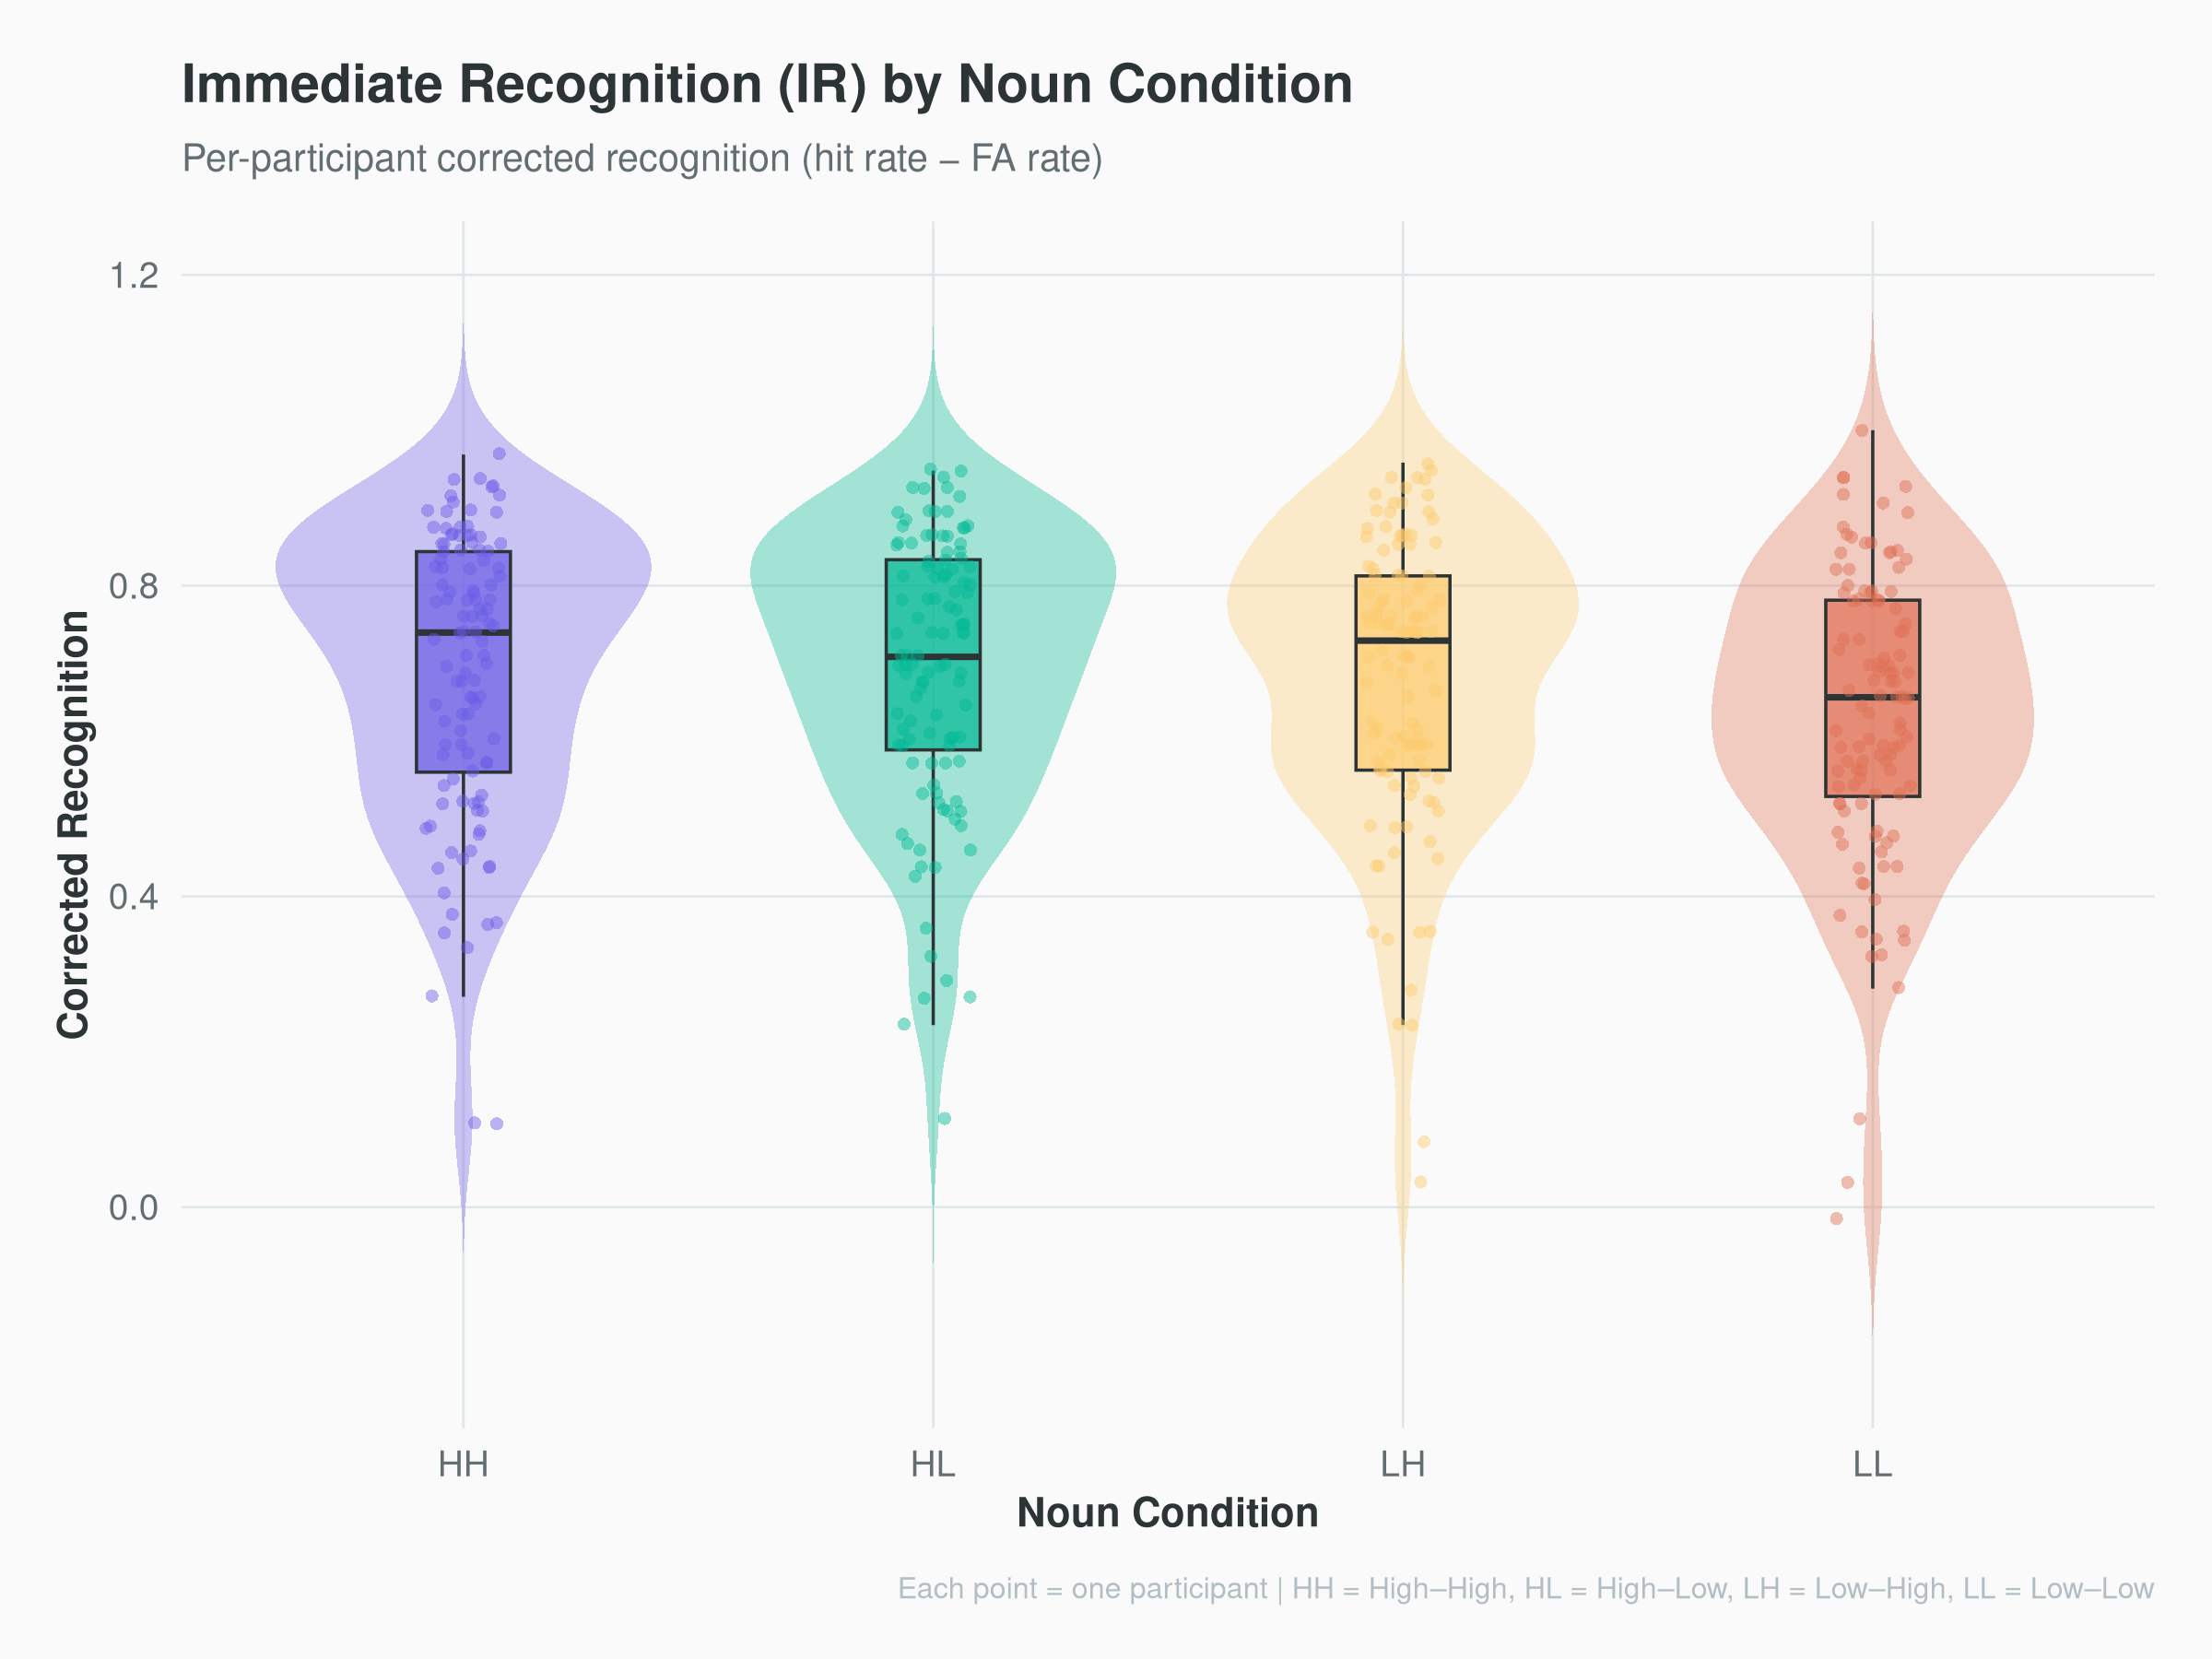
\includegraphics[width=\linewidth]{../../plots/01_ir_by_condition.png}
        \caption{Main effect of noun condition on corrected IR. Violin contours
        show the full participant-level distribution; boxes show interquartile
        range; points show individual participants. The LL condition is the only
        one with a visibly depressed distribution.}
        \label{fig:ir_condition}
    \end{minipage}\hfill
    \begin{minipage}{0.48\textwidth}
        \centering
        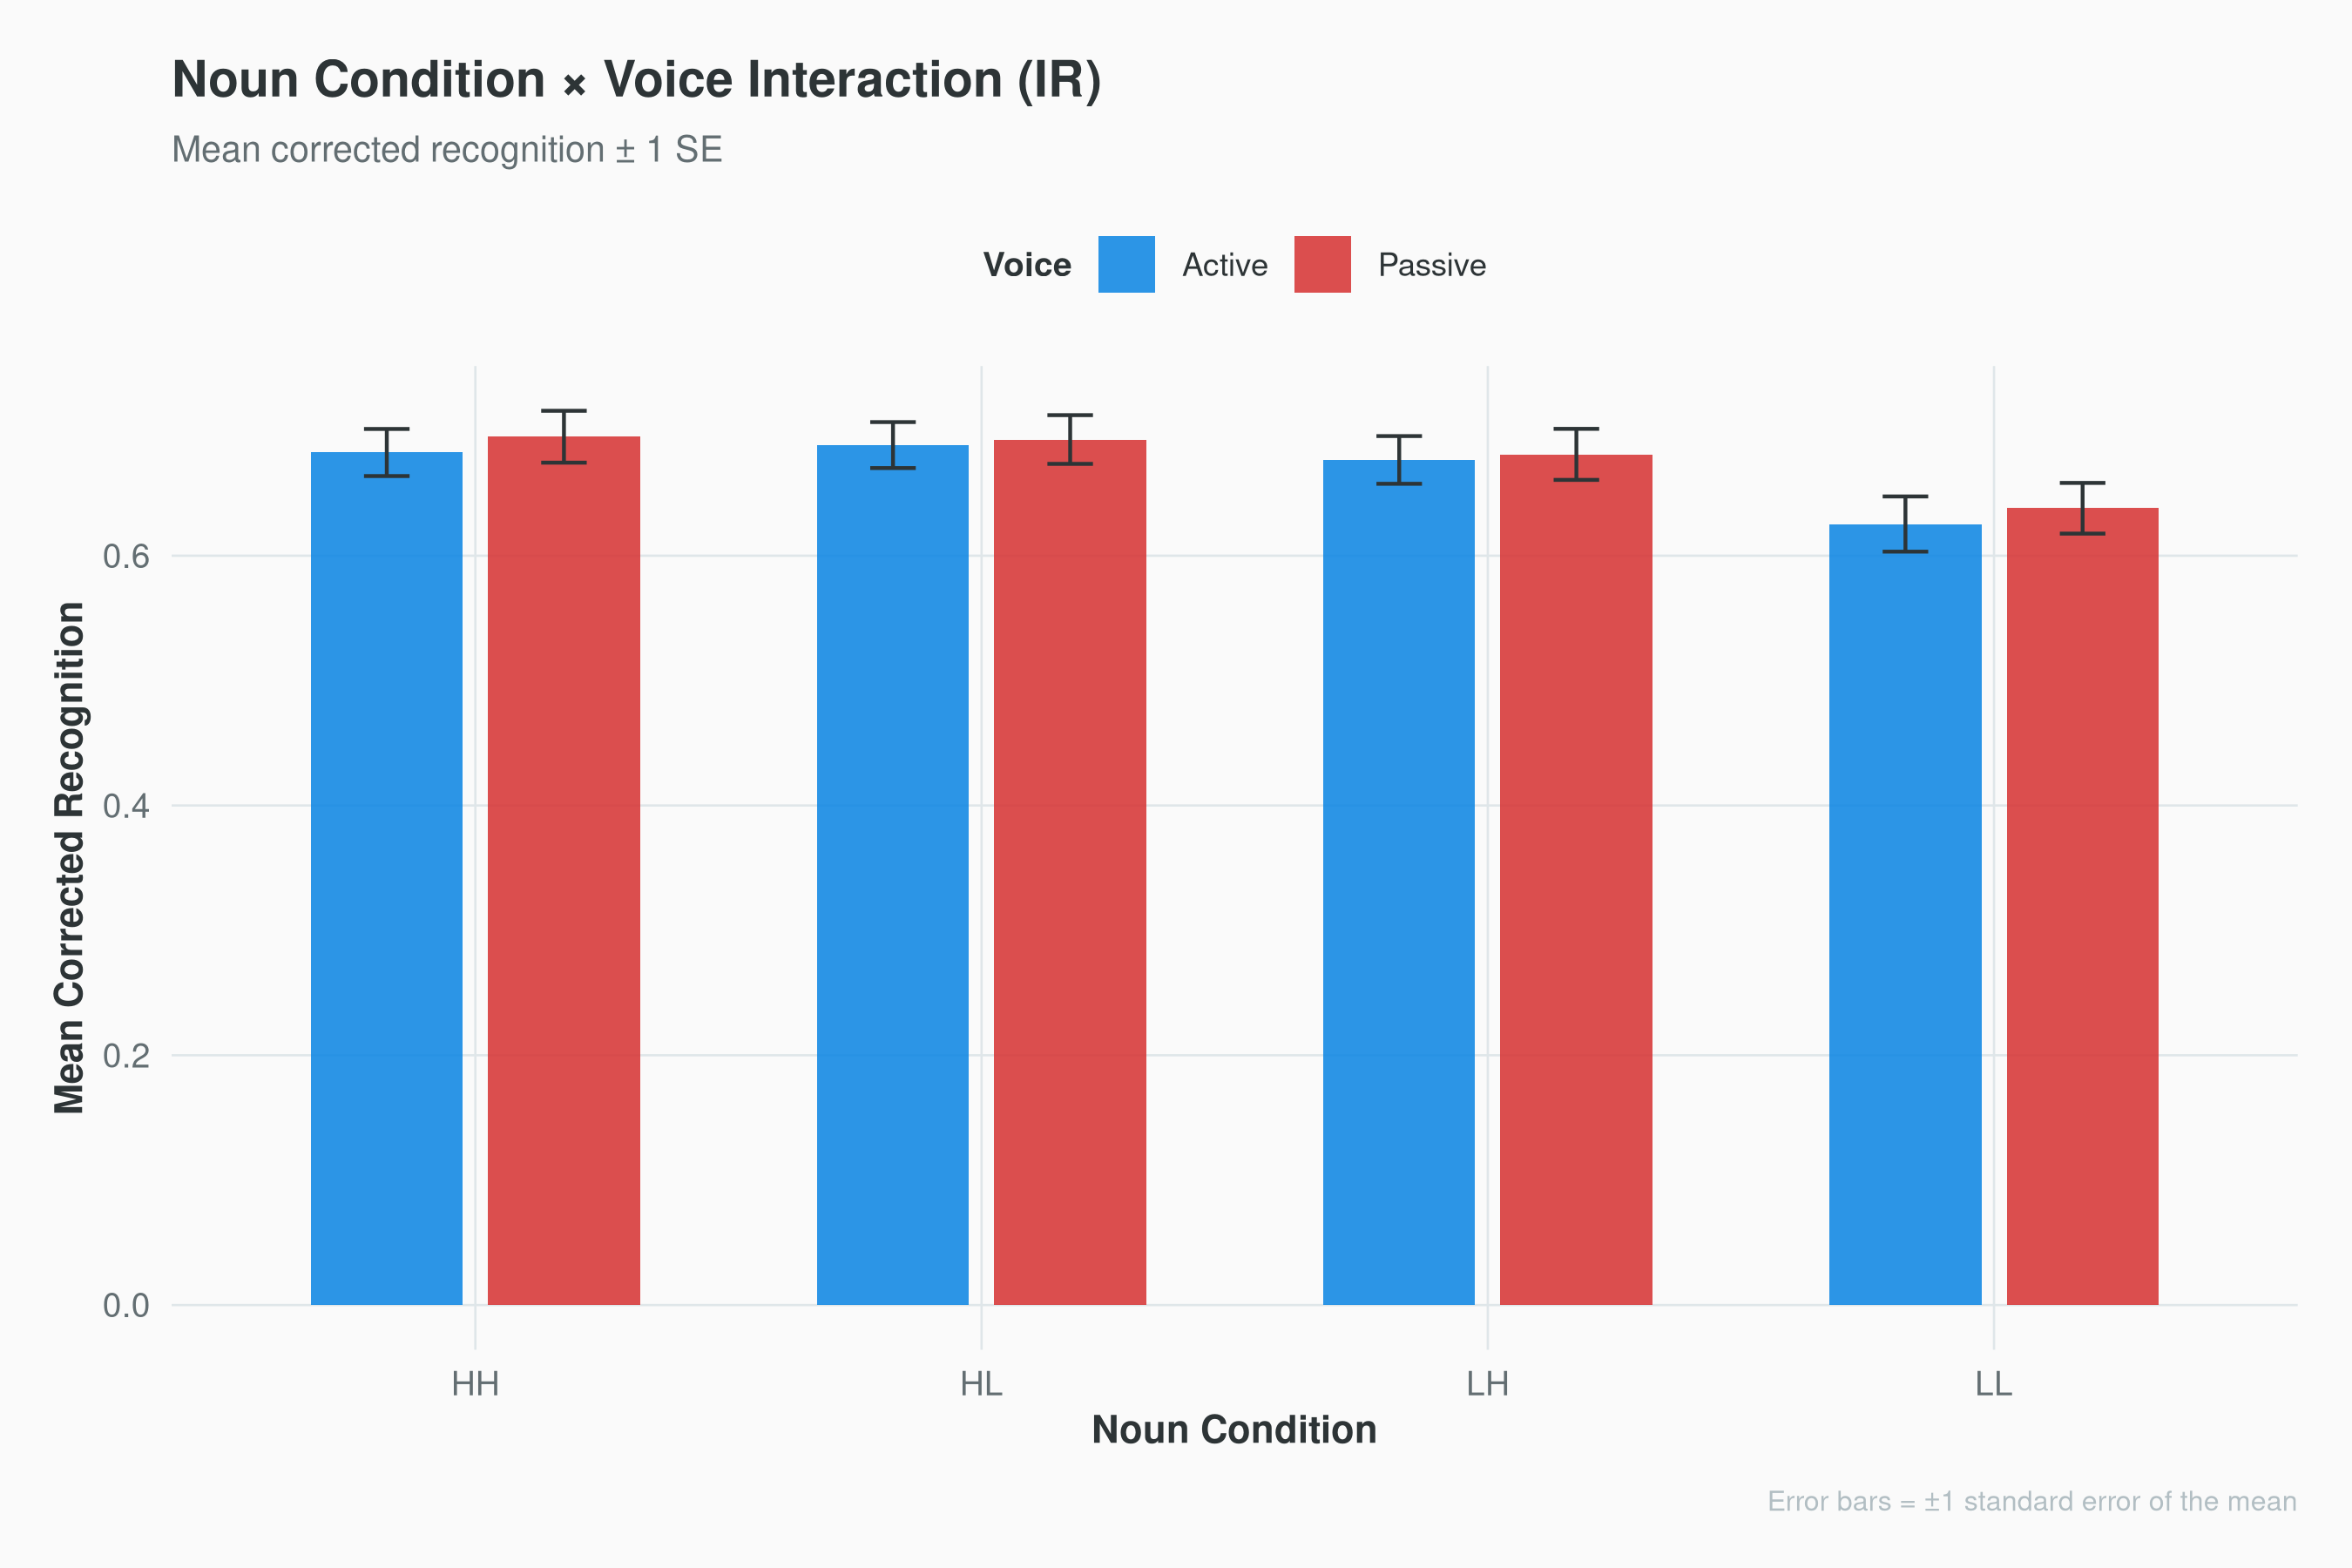
\includegraphics[width=\linewidth]{../../plots/03_ir_condition_x_voice.png}
        \caption{Mean corrected IR ($\pm 1$ SE) across the 8 noun-condition
        $\times$ voice cells. The LL disadvantage replicates within both active
        and passive voice, with no evidence of an interaction.}
        \label{fig:ir_voice}
    \end{minipage}
\end{figure}


\subsection{Noun Condition Does Not Affect Wording Recognition}

In contrast to the IR result, a Kruskal-Wallis test found no significant effect
of noun condition on WR accuracy, $H(3) = 1.98$, $p = .576$
(Figure~\ref{fig:wr_condition}). Mean WR accuracy by condition is presented in
Table~\ref{tab:wr}. Despite the large spread in IR scores across conditions,
participants were equally accurate at discriminating grammatical voice regardless
of noun imageability. This null result — for WR but not IR — supports the
prediction derived from \citeauthor{begg1971}'s (\citeyear{begg1971}) dual-trace
model: noun imageability specifically influences the richness of the semantic gist
image, while the representation underlying voice discrimination operates through
independent mechanisms and is insensitive to the imagistic quality of the
constituent words.

\begin{table}[H]
\centering
\caption{Wording Recognition (WR) Accuracy by Noun Condition ($n = 112$)}
\label{tab:wr}
\begin{tabular}{@{}lccc@{}}
\toprule
Condition & $M$ & $SD$ & Note \\ \midrule
HH & 0.748 & 0.151 & above chance \\
HL & 0.747 & 0.145 & above chance \\
LH & 0.762 & 0.160 & above chance \\
LL & 0.730 & 0.173 & above chance \\ \bottomrule
\end{tabular}
\end{table}

\begin{figure}[H]
    \centering
    \begin{minipage}{0.48\textwidth}
        \centering
        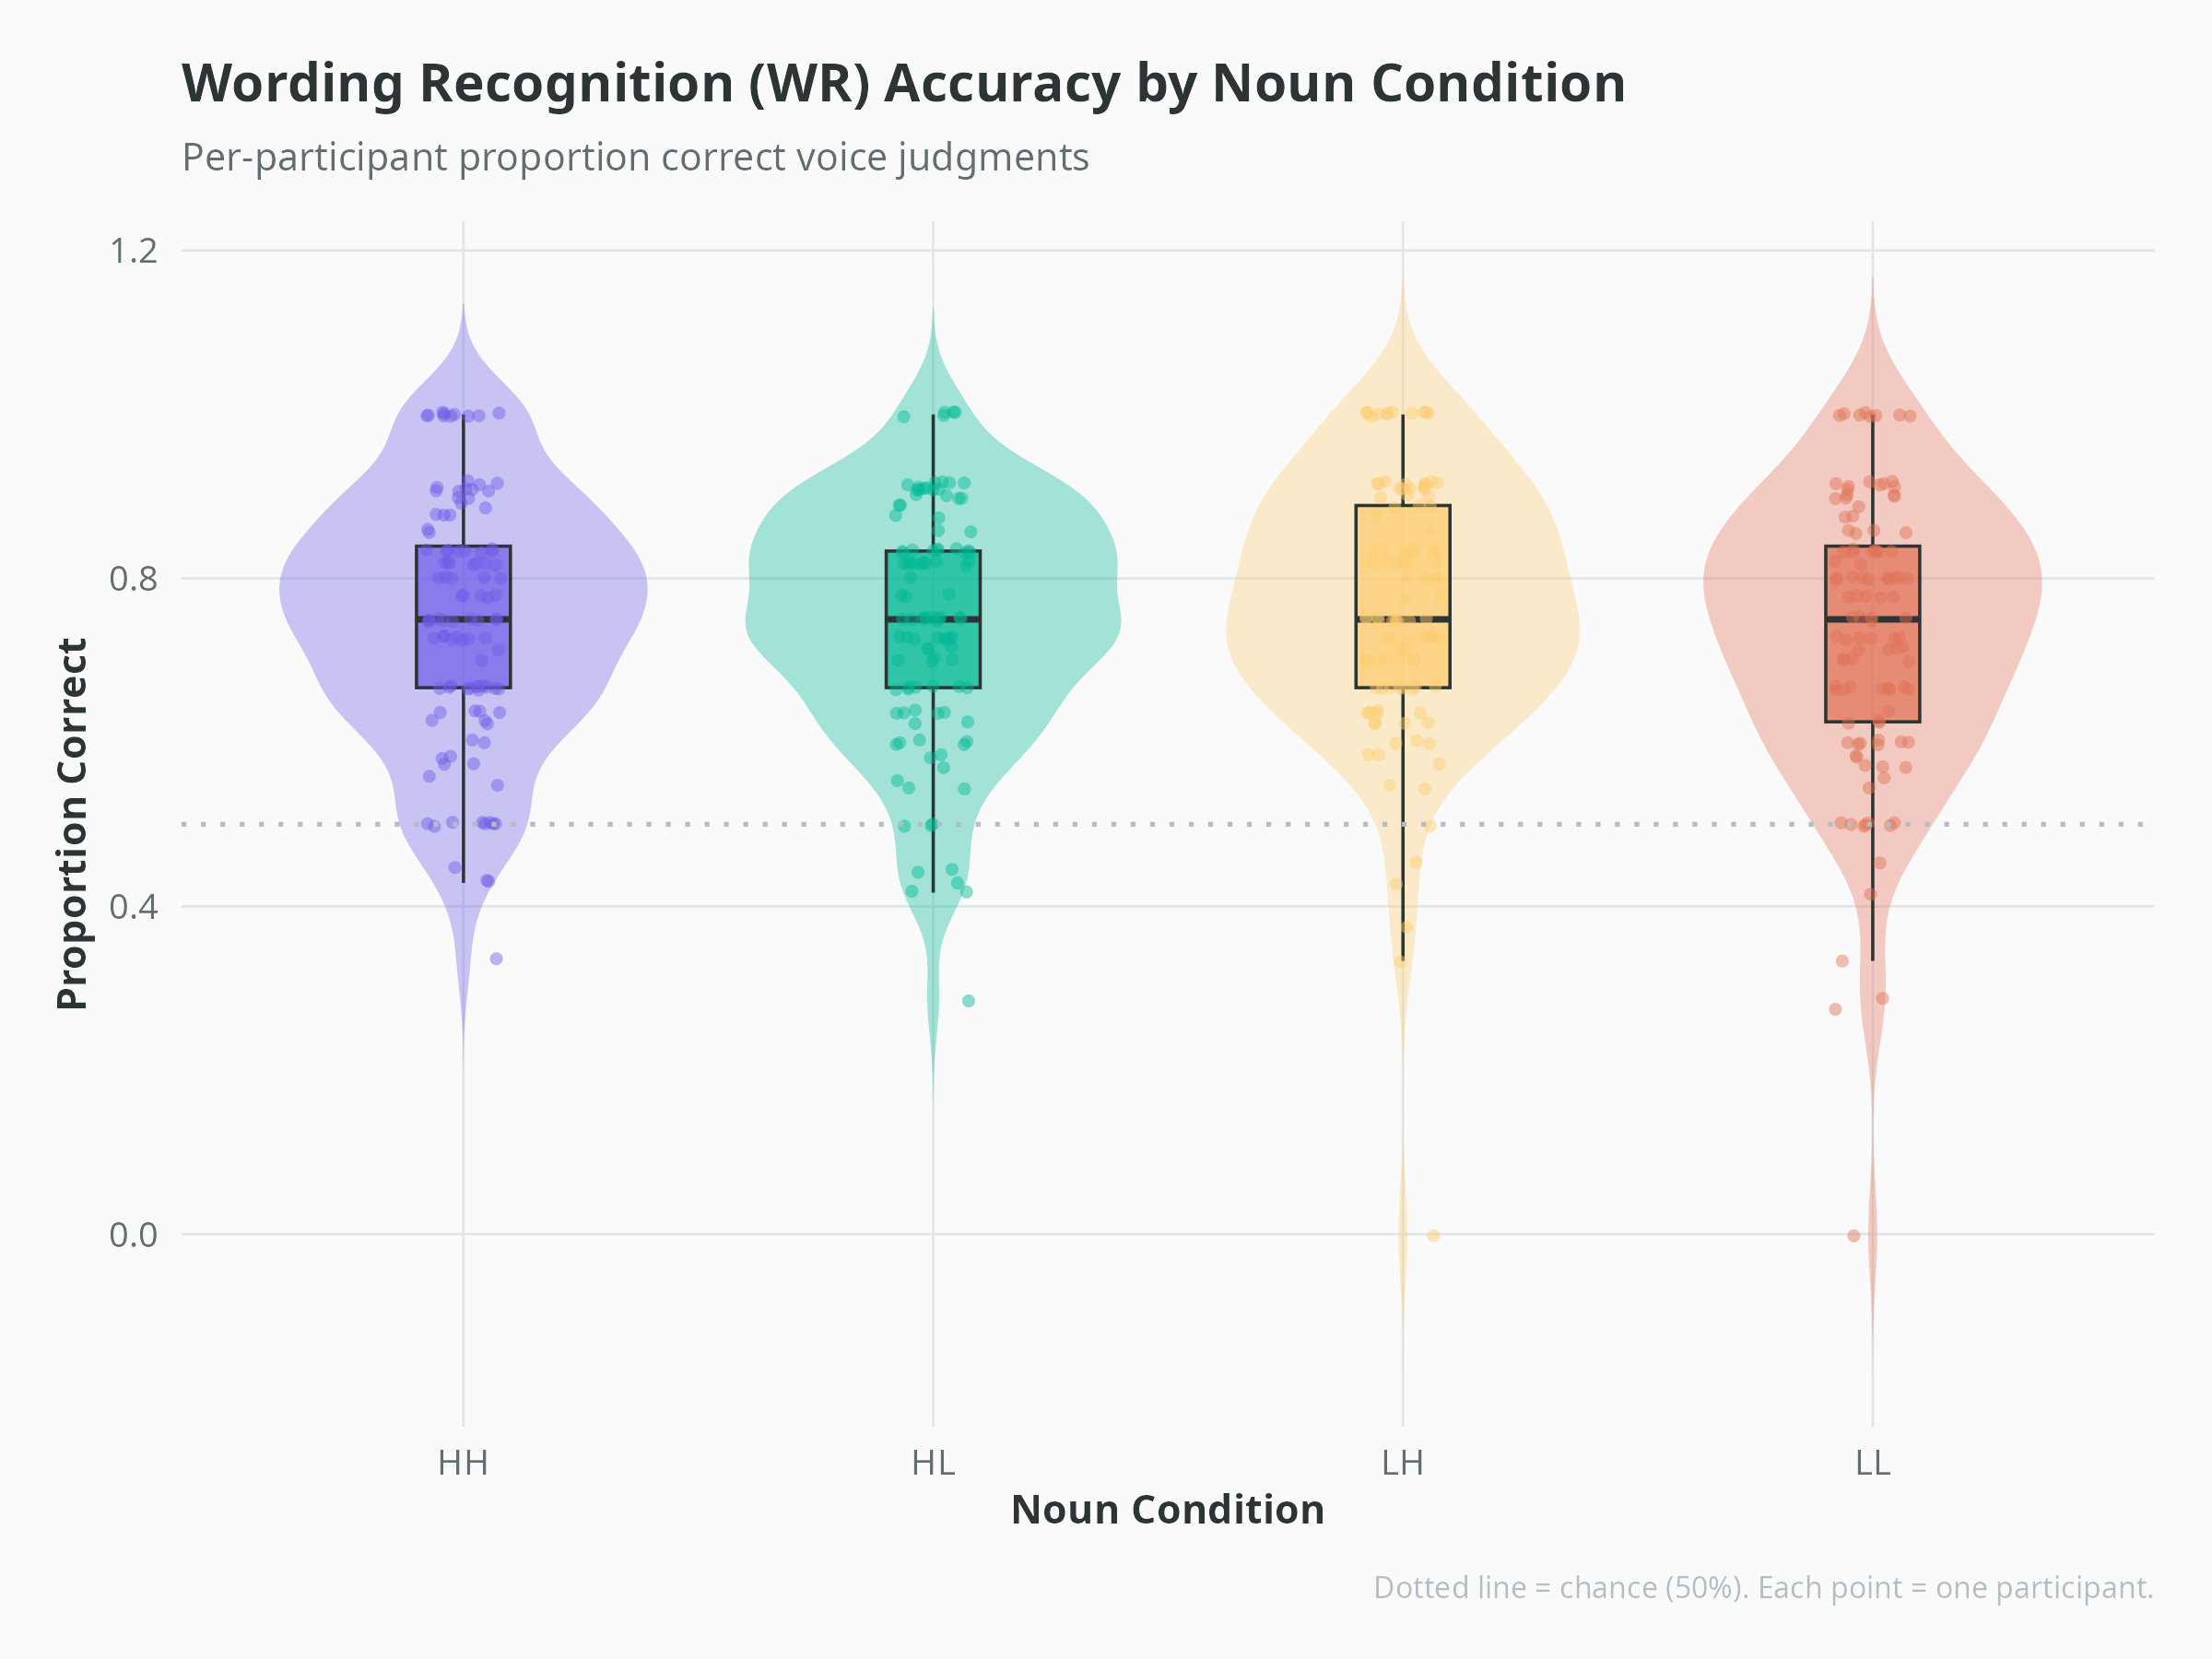
\includegraphics[width=\linewidth]{../../plots/02_wr_by_condition.png}
        \caption{WR accuracy by noun condition. All four distributions are clearly
        above the 0.50 chance line (dotted), confirming that participants retained
        surface-form information. No significant condition differences were found
        ($H(3) = 1.98$, $p = .576$).}
        \label{fig:wr_condition}
    \end{minipage}\hfill
    \begin{minipage}{0.48\textwidth}
        \centering
        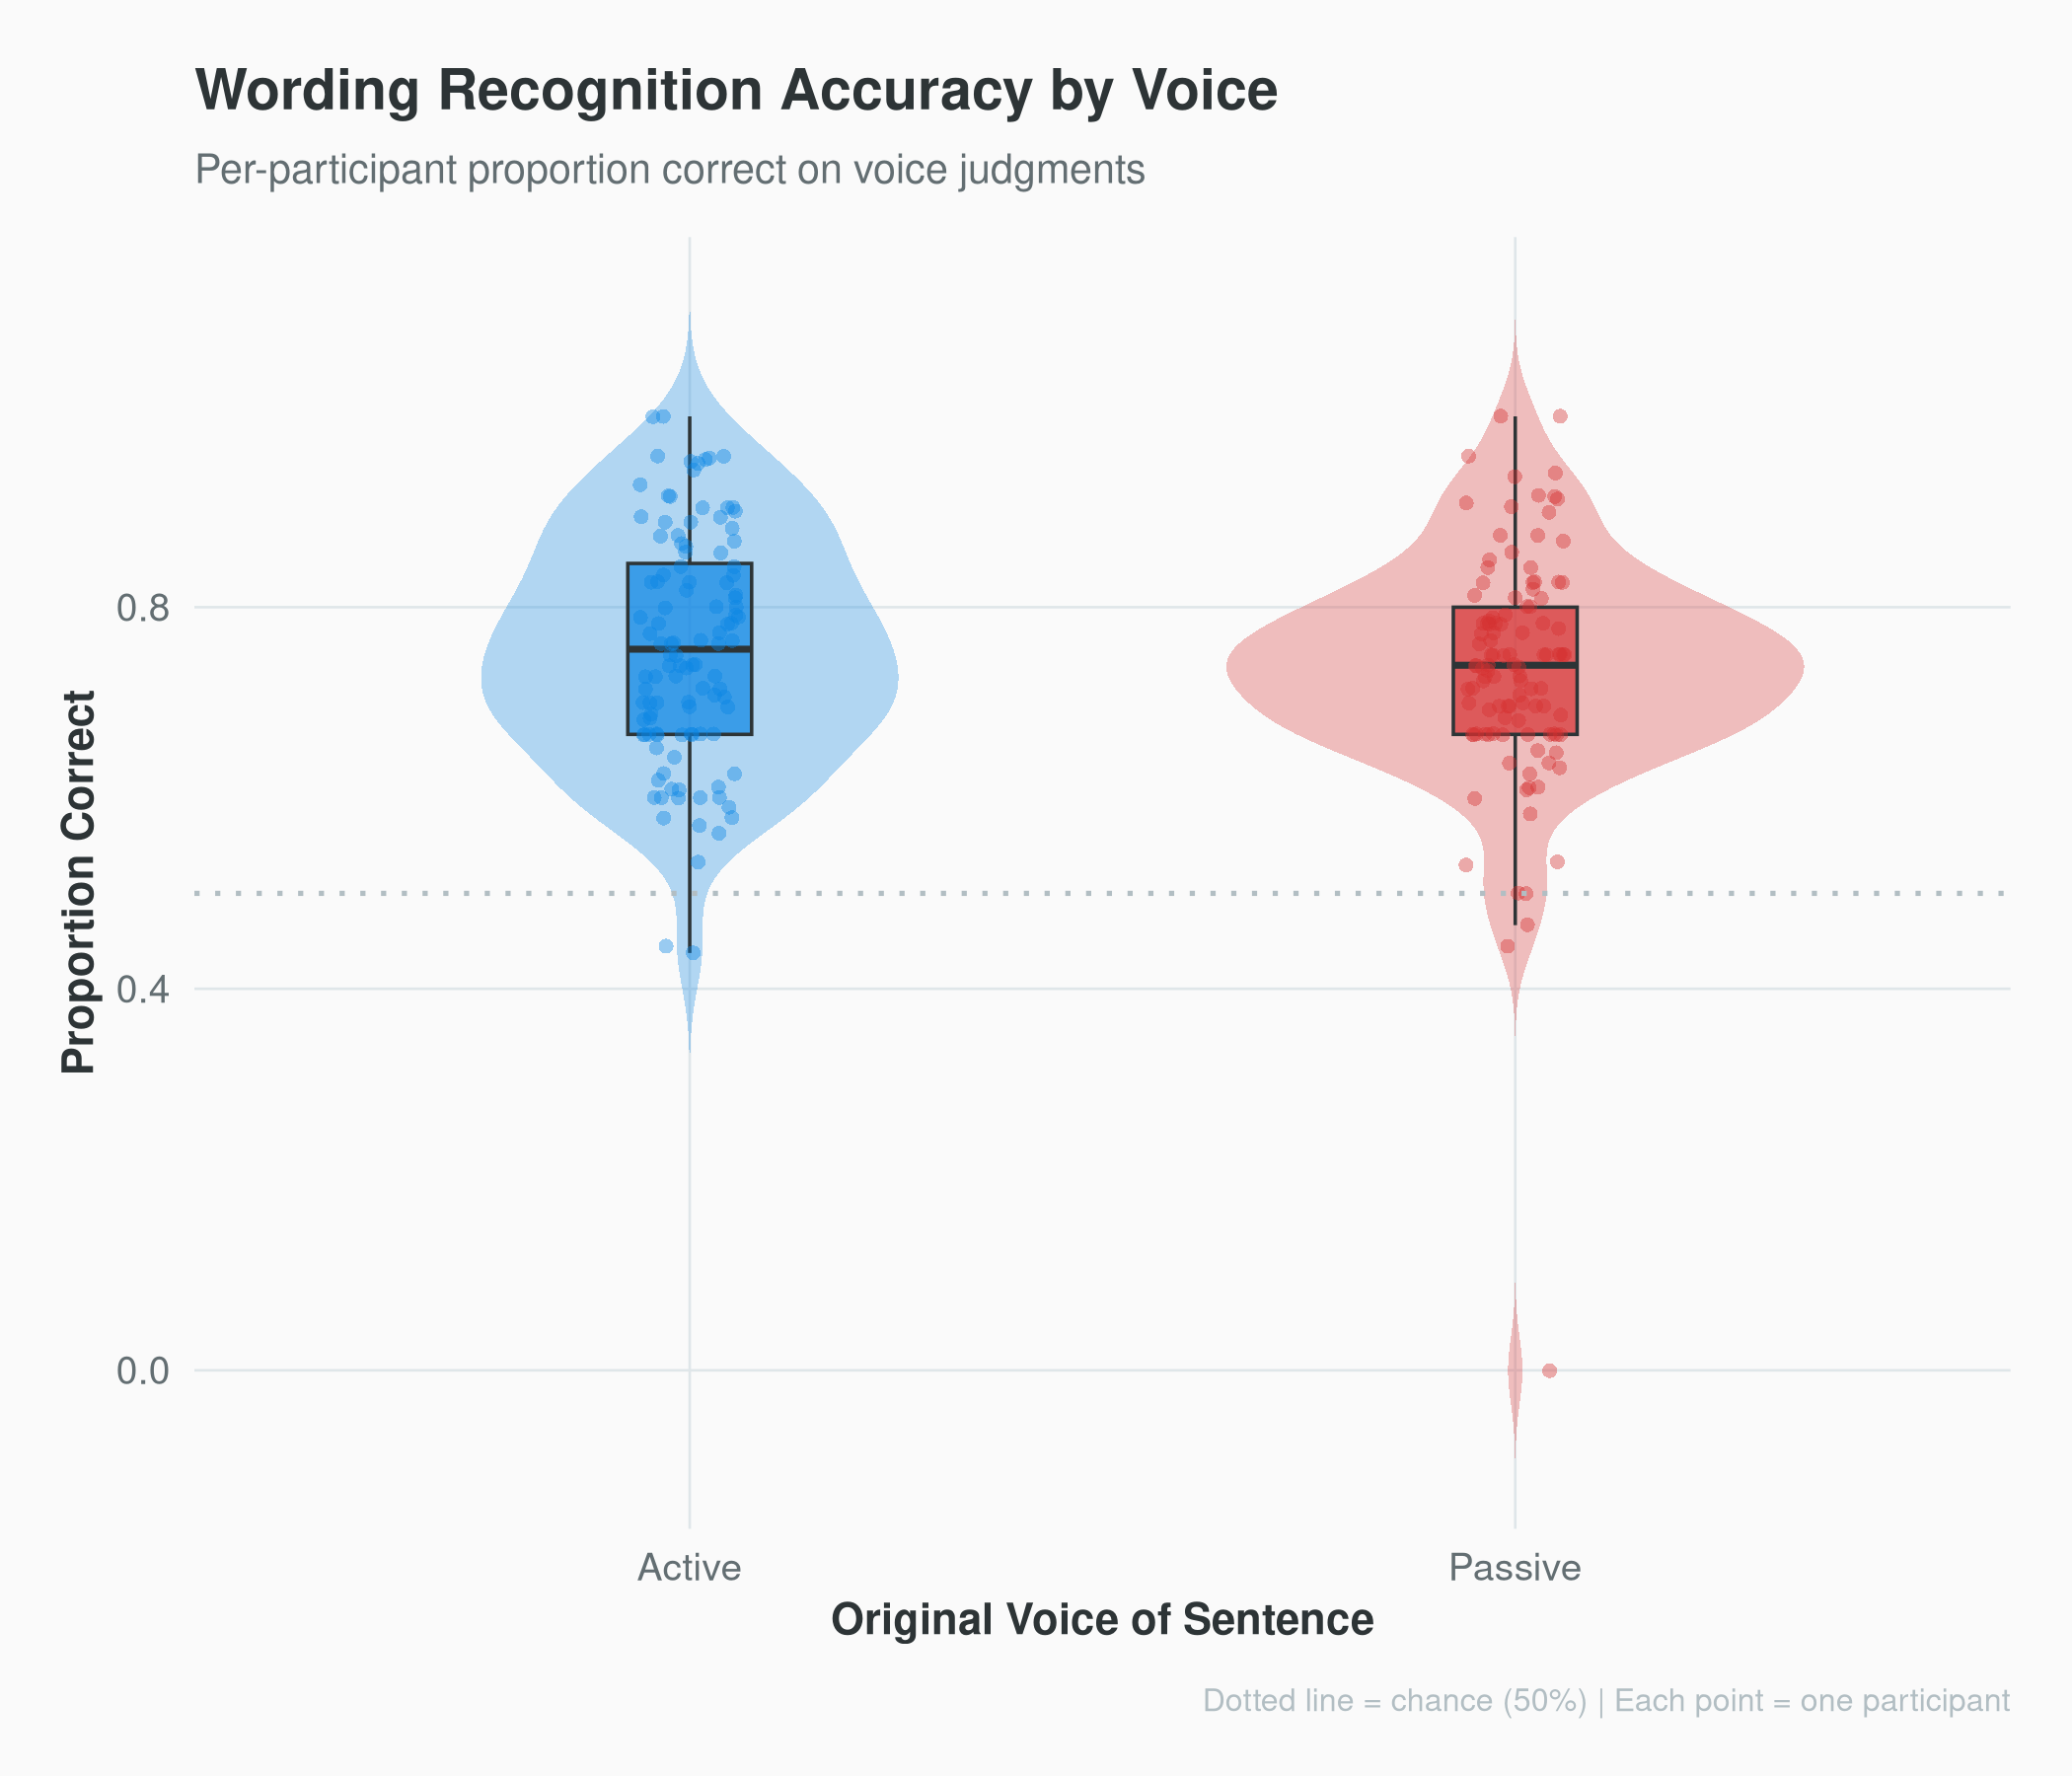
\includegraphics[width=\linewidth]{../../plots/11_wr_accuracy_by_voice.png}
        \caption{WR accuracy by grammatical voice. Both voices are well above
        chance. The numerical advantage for Active ($M = 0.757$) over Passive
        ($M = 0.735$) did not reach significance ($V = 3279$, $p = .113$).}
        \label{fig:wr_voice}
    \end{minipage}
\end{figure}


\subsection{Voice Effects on IR and WR}

\paragraph{Effect of voice on IR.}
A paired Wilcoxon signed-rank test found no significant main effect of
grammatical voice on corrected IR: $V = 1704$, $p = .374$ (Active $M = 0.668$,
$SD = 0.166$; Passive $M = 0.677$, $SD = 0.175$; Figures~\ref{fig:ir_voice}
and~\ref{fig:voice_slope}). Whether a sentence was encoded in active or passive
voice had no measurable effect on how well its meaning was recognised — a direct
replication of \citeauthor{begg1971}'s (\citeyear{begg1971}) finding that meaning
recognition is equally accurate for paraphrase and identical-wording probes.
The 8-cell means in Table~\ref{tab:8cell} confirm that the noun-condition
threshold effect replicates consistently within both voice conditions, with no
evidence of a differential interaction.

\begin{table}[H]
\centering
\caption{Mean Corrected IR by Noun Condition $\times$ Voice ($n = 112$ per cell)}
\label{tab:8cell}
\begin{tabular}{@{}lcccc@{}}
\toprule
Condition & Active $M$ & Active $SD$ & Passive $M$ & Passive $SD$ \\ \midrule
HH & 0.683 & 0.199 & 0.695 & 0.220 \\
HL & 0.689 & 0.195 & 0.693 & 0.206 \\
LH & 0.677 & 0.202 & 0.681 & 0.216 \\
LL & 0.625 & 0.234 & 0.638 & 0.215 \\ \bottomrule
\end{tabular}
\end{table}

\paragraph{Effect of voice on WR.}
WR accuracy was numerically higher for active-voice sentences ($M = 0.757$,
$SD = 0.120$) than passive-voice sentences ($M = 0.735$, $SD = 0.127$), but
this difference did not reach statistical significance: $V = 3279$, $p = .113$
(Figure~\ref{fig:wr_voice}). Critically, one-sample Wilcoxon tests confirmed
that both voices were reliably above chance: Active $V = 6322$, $p < .001$;
Passive $V = 5990$, $p < .001$. Participants could accurately detect voice
mismatches regardless of the original grammatical form — consistent with
\citeauthor{bregman1968}'s (\citeyear{bregman1968}) finding that above-chance
second-guess accuracy for the active--passive distinction persists even after
the verbatim trace has partially degraded. The non-significant trend favouring
active-voice WR is directionally consistent with the active-construction bias
documented by \citet{james1973} and merits re-examination with the full sample
in Report 2.

\begin{figure}[H]
    \centering
    \begin{minipage}{0.48\textwidth}
        \centering
        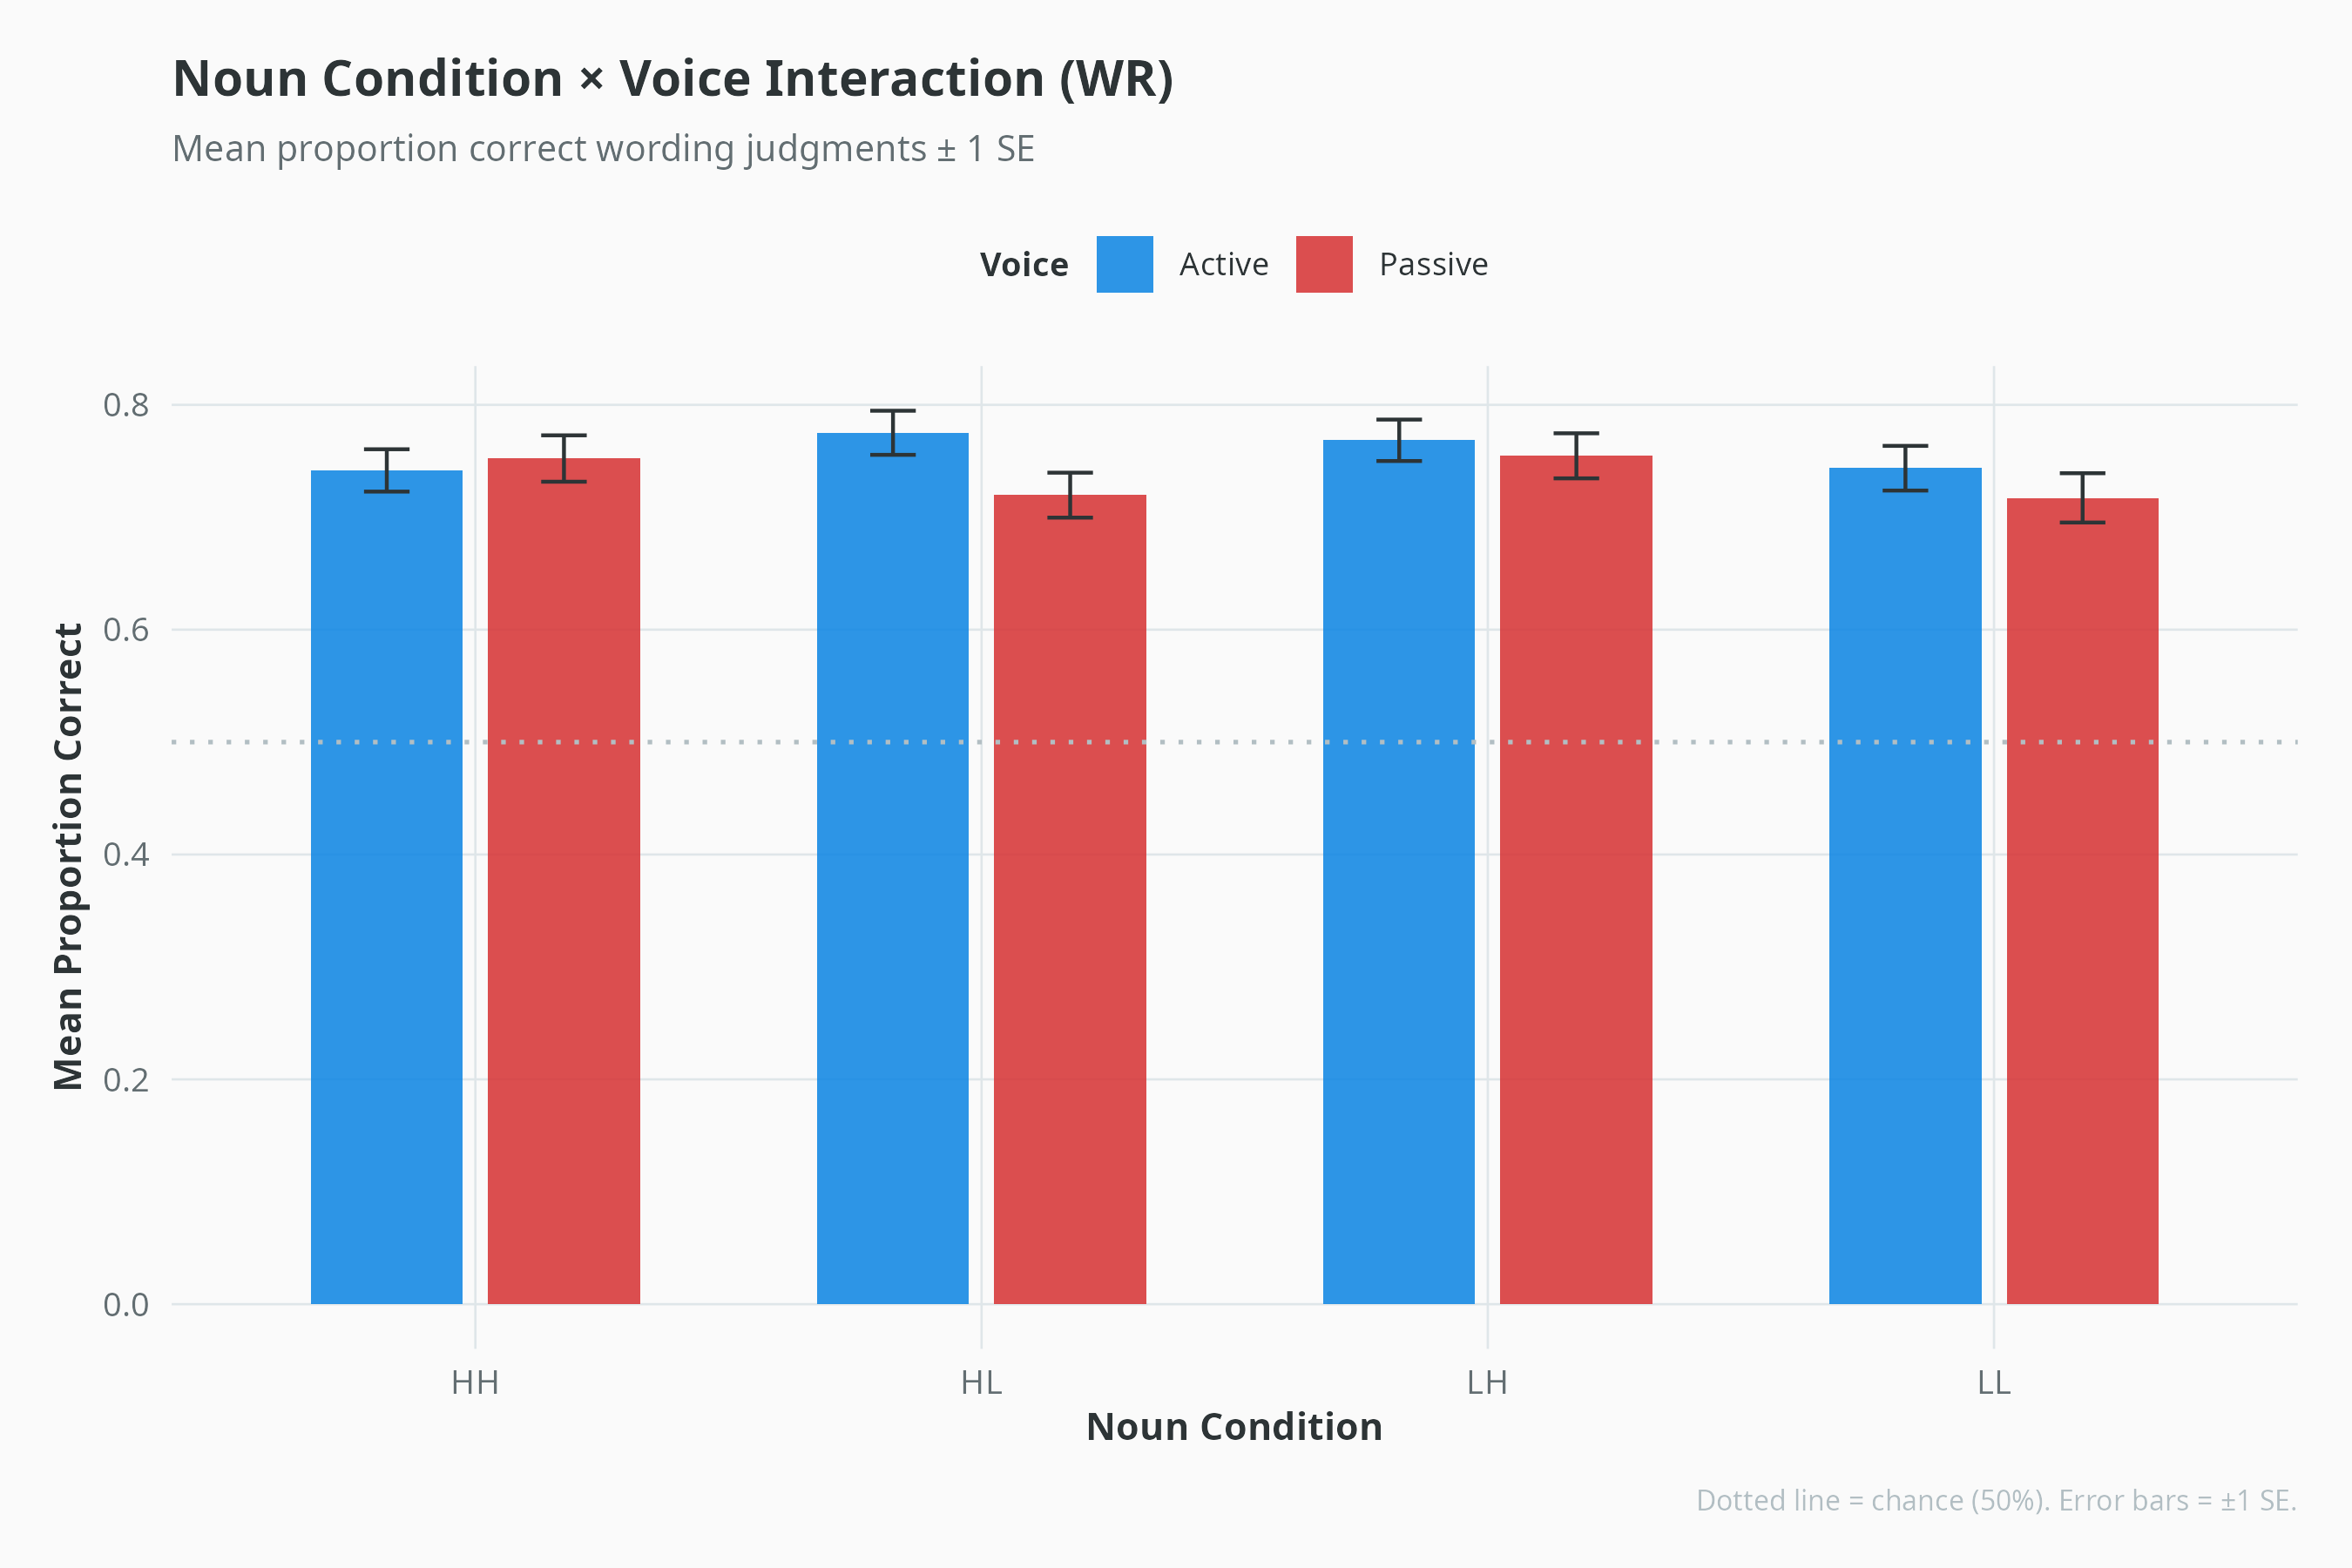
\includegraphics[width=\linewidth]{../../plots/04_wr_condition_x_voice.png}
        \caption{Mean WR accuracy ($\pm 1$ SE) across 8 noun-condition $\times$
        voice cells. Performance is uniformly high across all cells with no
        discernible interaction, consistent with the null noun-condition effect
        on WR.}
        \label{fig:wr_interaction}
    \end{minipage}\hfill
    \begin{minipage}{0.48\textwidth}
        \centering
        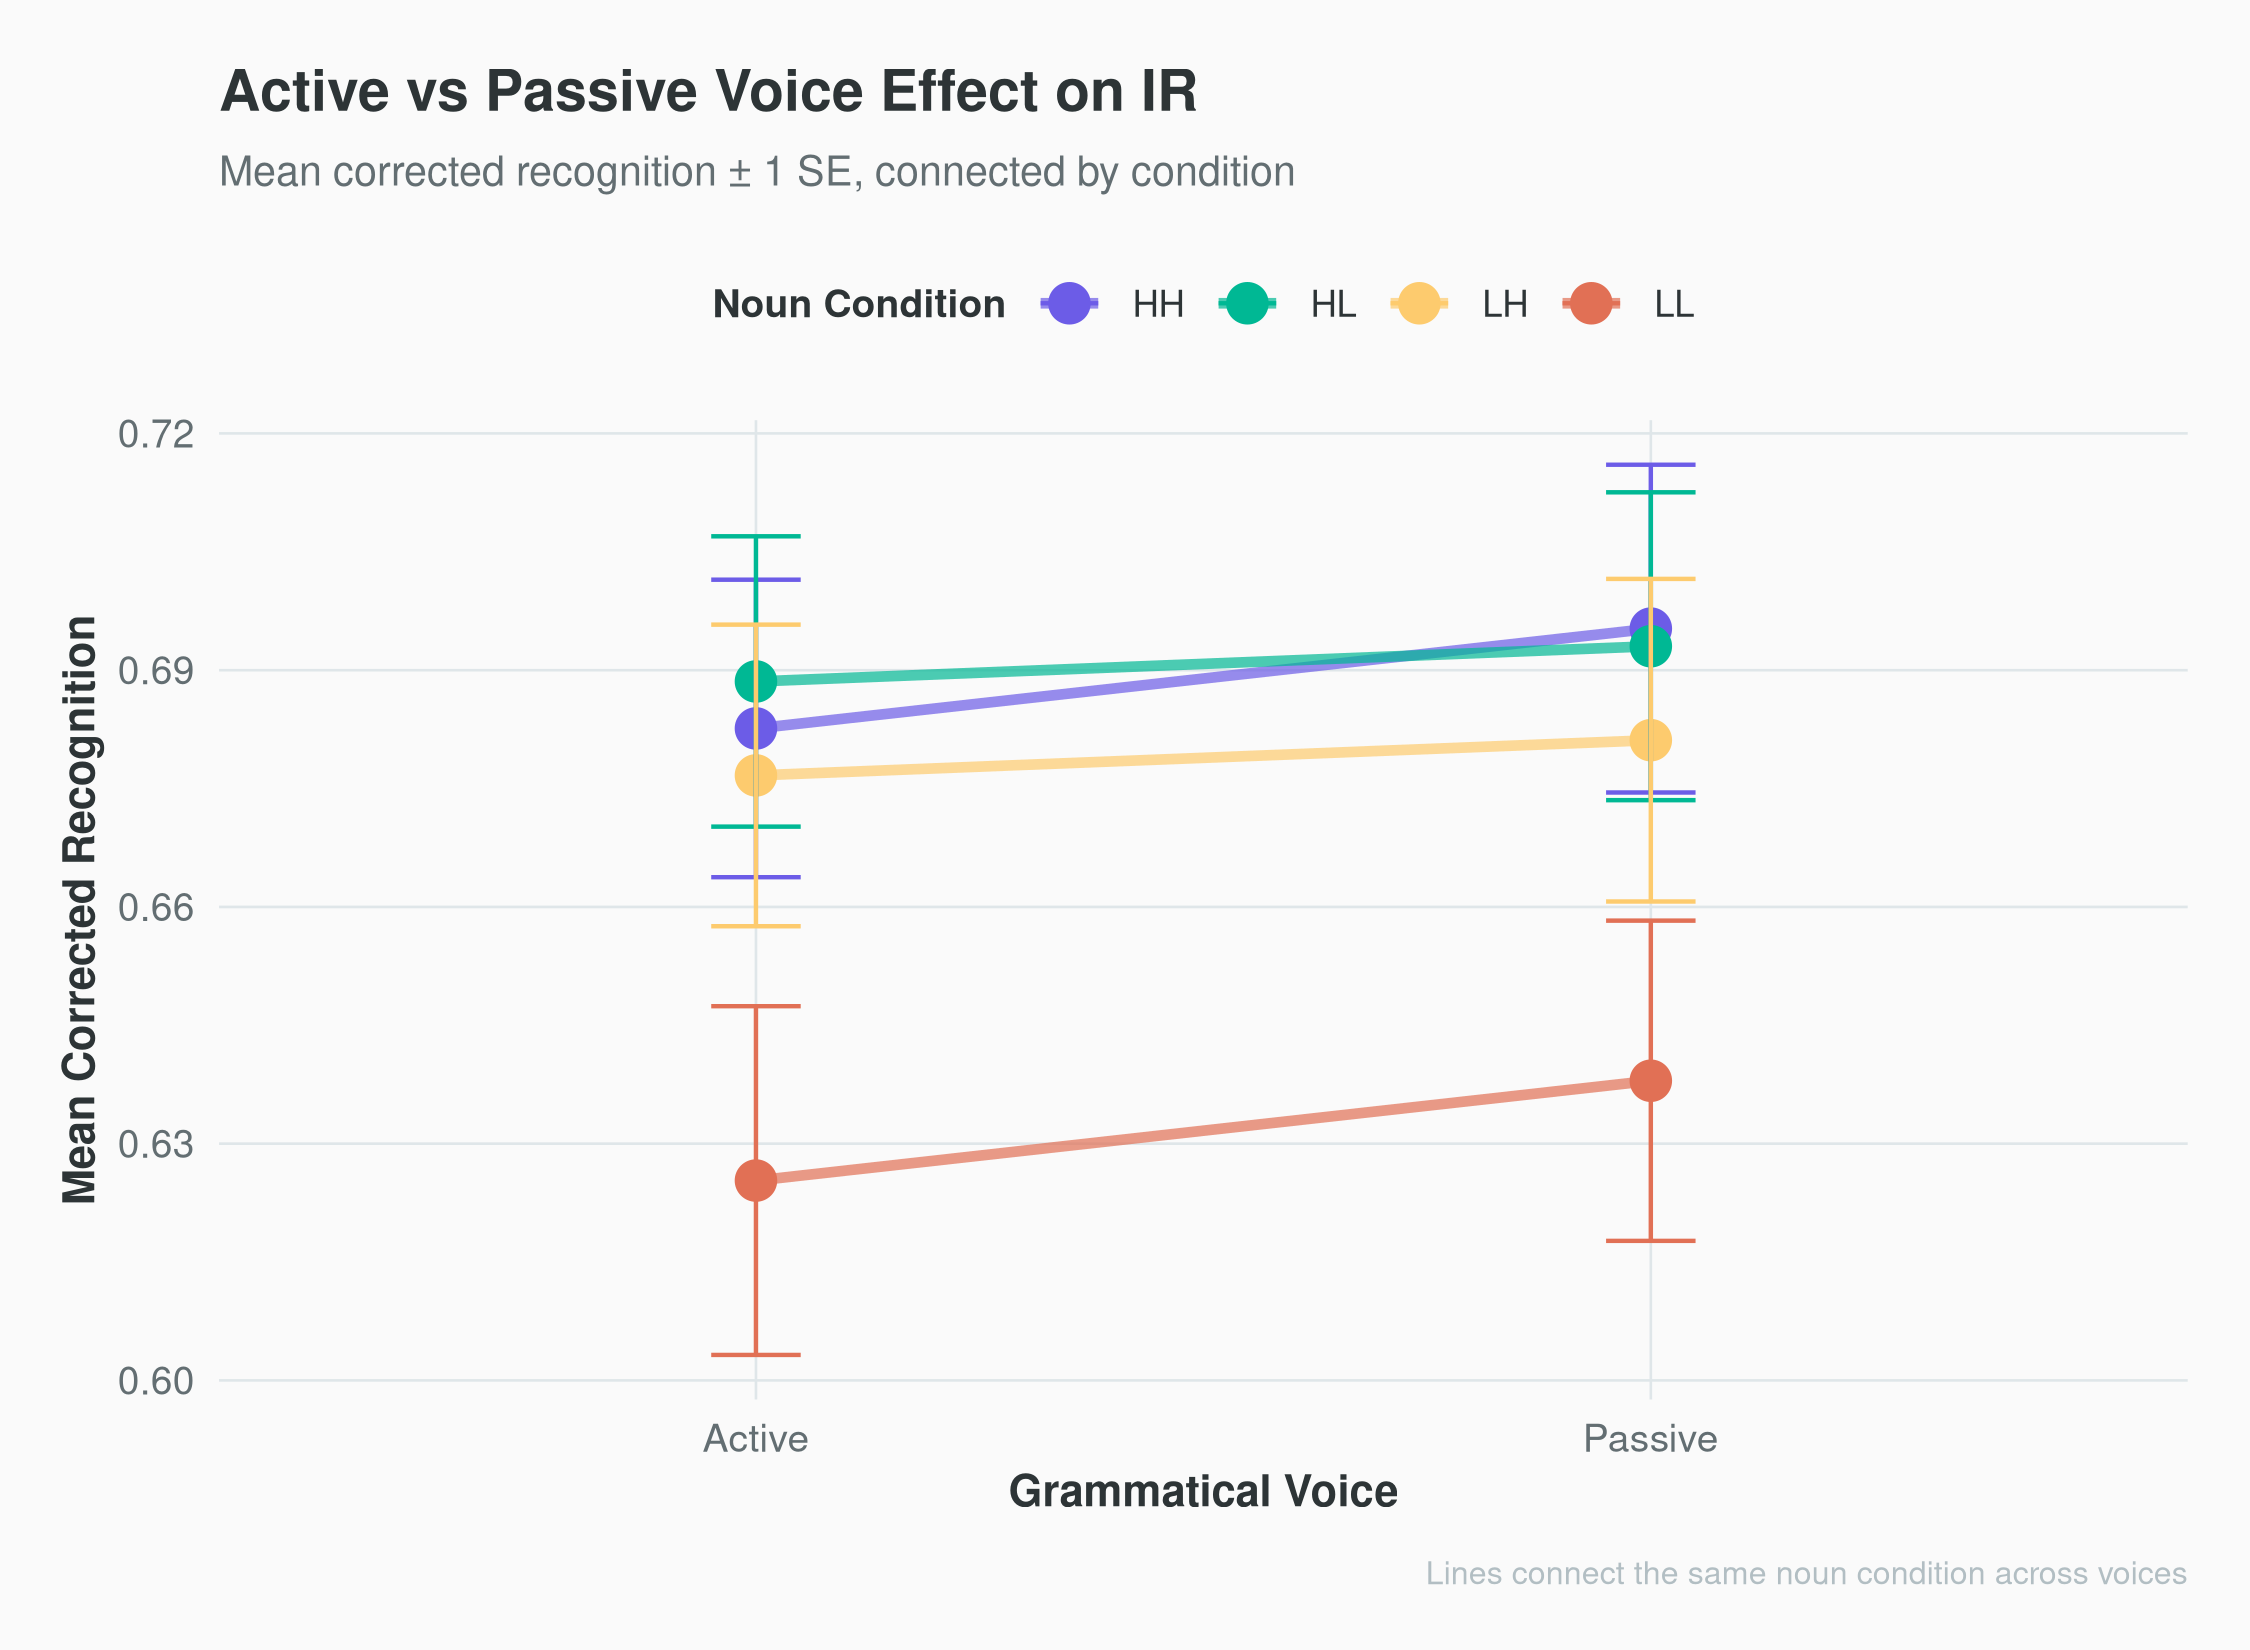
\includegraphics[width=\linewidth]{../../plots/09_voice_slope.png}
        \caption{Voice slope graph for IR. Near-parallel lines indicate that the
        absence of a voice effect generalises across all four noun conditions,
        with no crossover interaction.}
        \label{fig:voice_slope}
    \end{minipage}
\end{figure}


\subsection{Relationship Between Meaning and Wording Memory}

Although IR and WR are predicted to operate on distinct memory representations
\citep{begg1971}, they were significantly and positively correlated at the
participant level (Spearman $\rho = .248$, $p < .001$;
Figure~\ref{fig:scatter_wr_ir}). Participants who more reliably recognised
sentence meaning also showed superior voice discrimination. The positive sign
of this association is consistent with \citeauthor{begg1971}'s
(\citeyear{begg1971}) observation that the product rule for stochastic
independence (\(P_{cM} \cdot P_{cW} \approx P_{cM\&W}\)) holds only
approximately: the two systems are largely but not entirely independent.
The modest magnitude (\(\rho = .25\)) confirms that the two memory systems
are not redundant, in line with the partially dissociable dual-trace account.

\begin{figure}[H]
    \centering
    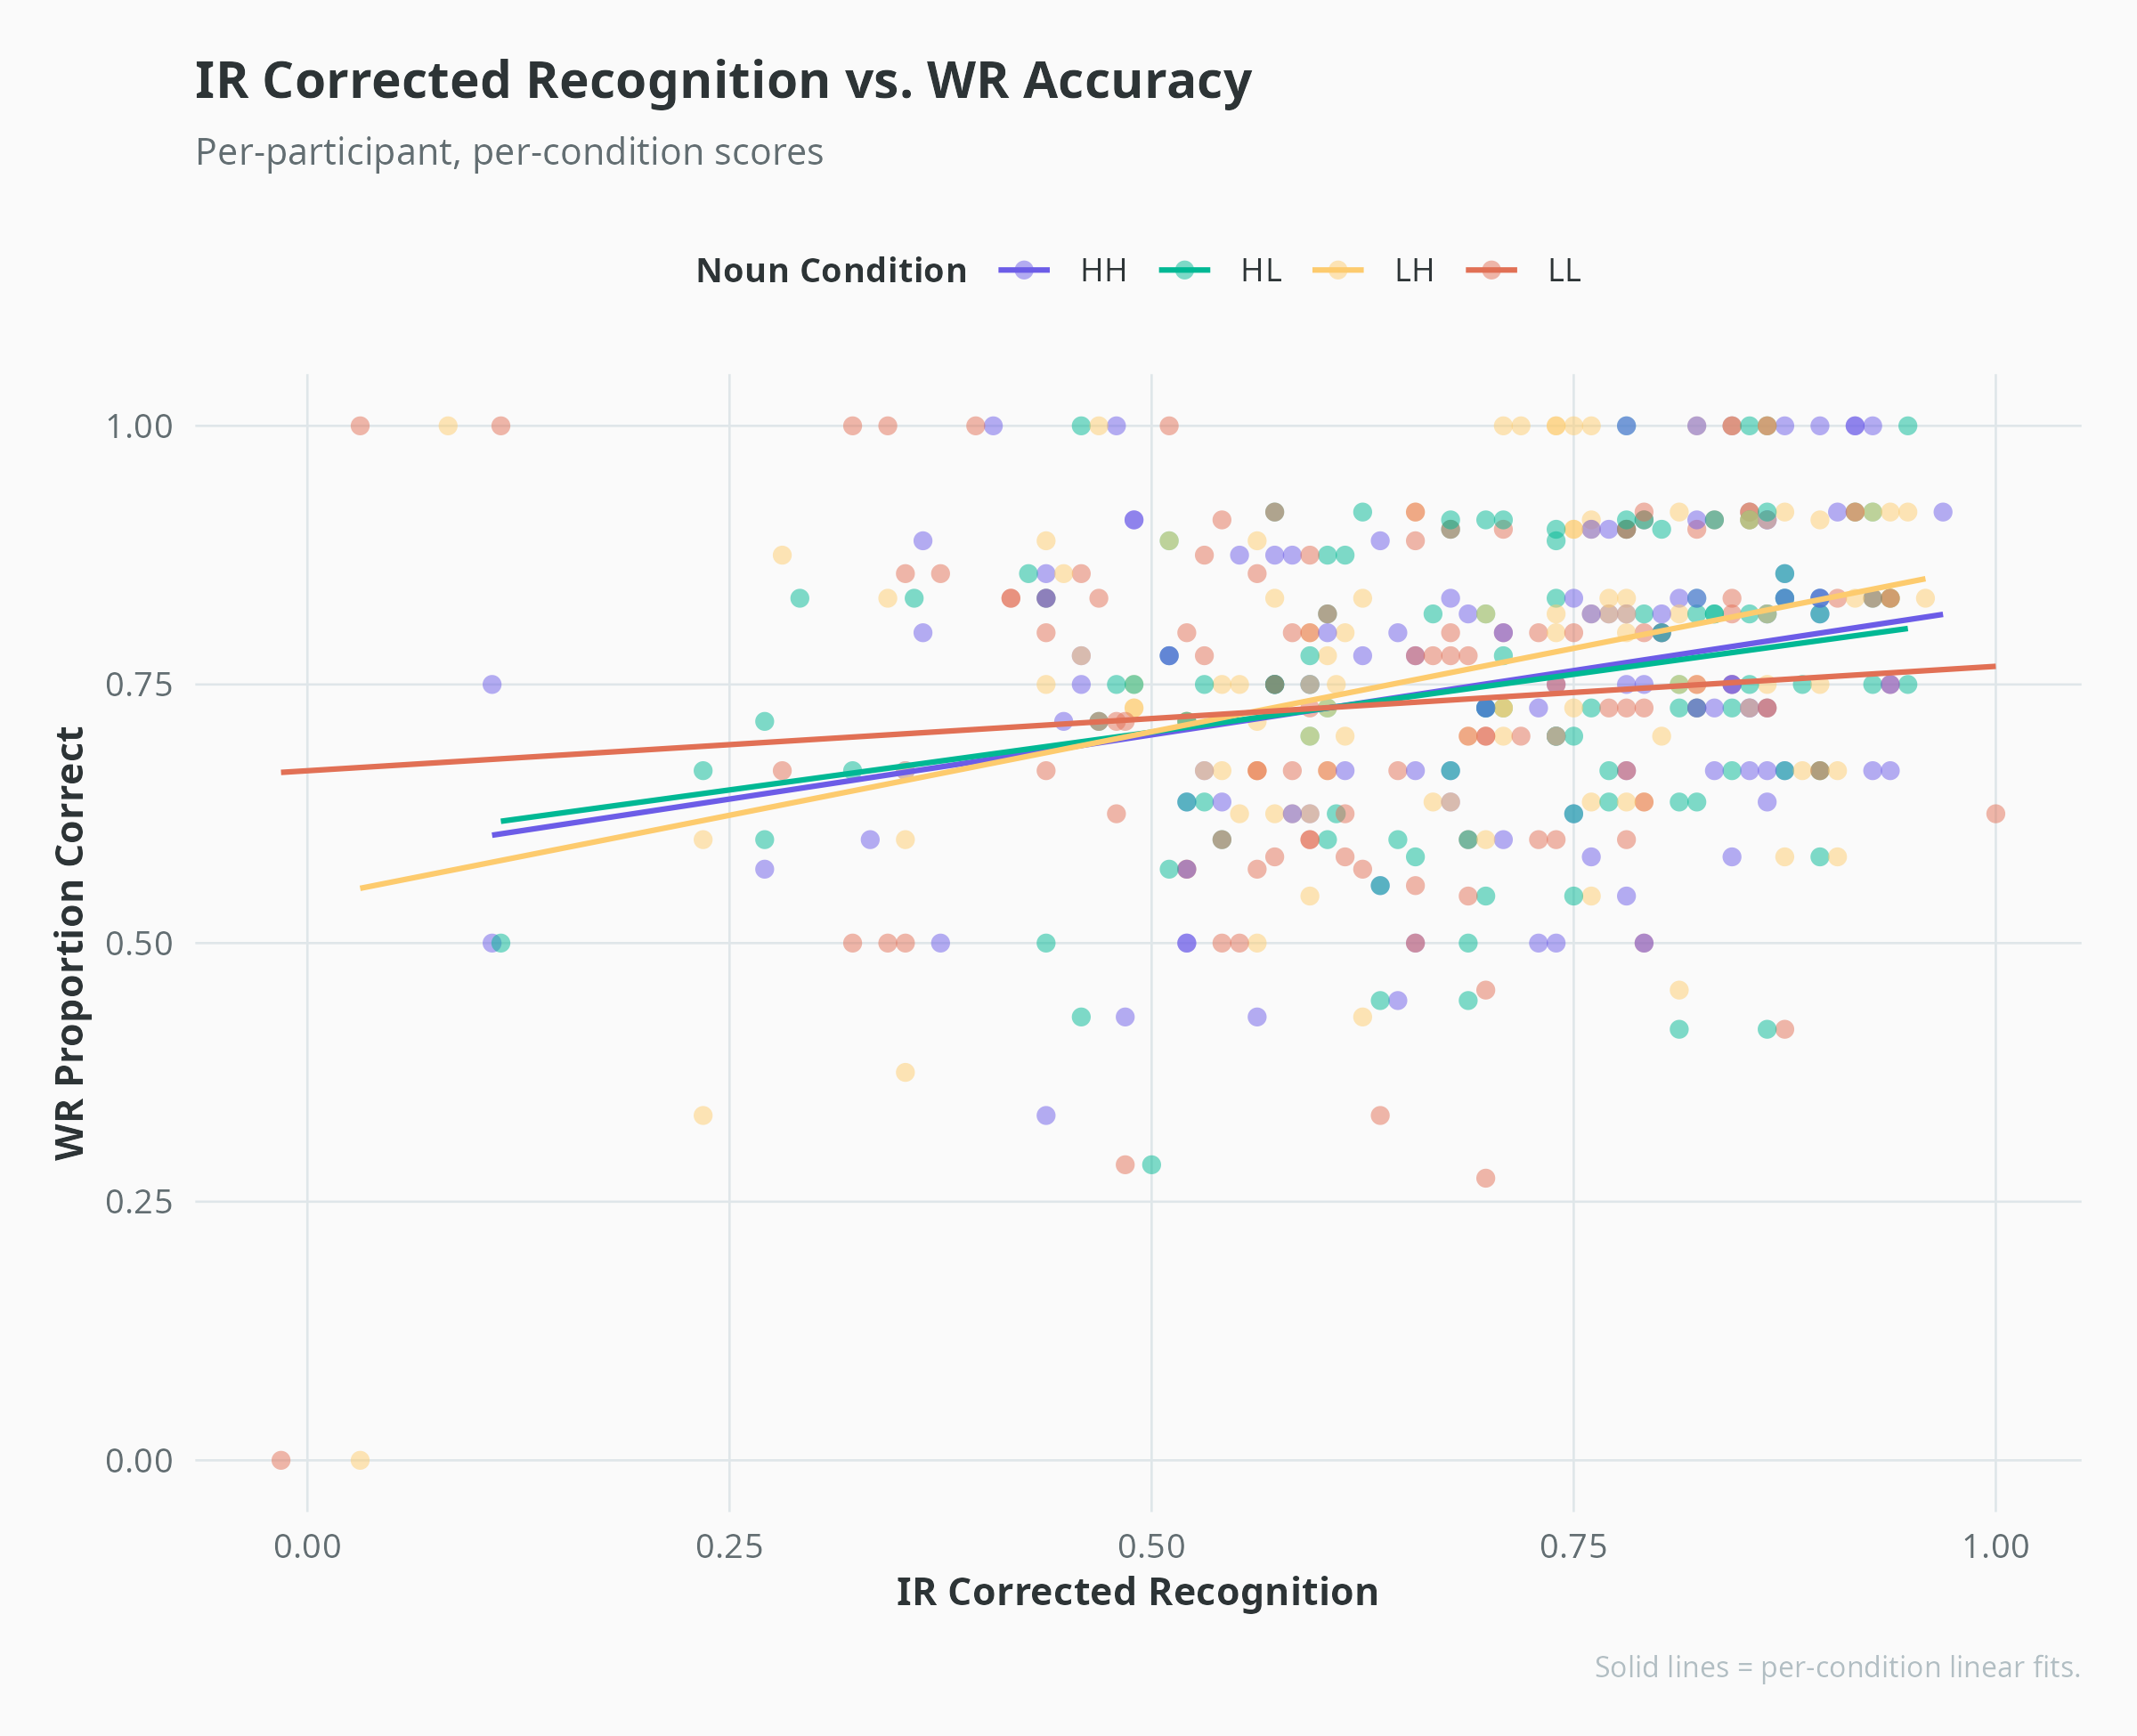
\includegraphics[width=0.6\textwidth]{../../plots/10_ir_vs_wr.png}
    \caption{Scatterplot of per-participant, per-condition corrected IR against
    WR accuracy (Spearman $\rho = .248$, $p < .001$). Separate linear fits are
    shown for each noun condition. The positive relationship suggests co-occurring
    encoding strengths; the modest effect size indicates partially dissociable
    representations, consistent with \citet{begg1971}.}
    \label{fig:scatter_wr_ir}
\end{figure}


\subsection{Reaction Time as a Supplementary Processing Index}

Mean IR reaction times by noun condition were: HH $M = 1{,}725$ ms ($SD = 319$),
HL $M = 1{,}729$ ms ($SD = 365$), LH $M = 1{,}677$ ms ($SD = 335$), and
LL $M = 1{,}762$ ms ($SD = 336$). A Kruskal-Wallis test found no significant
effect, $H(3) = 4.44$, $p = .218$ (Figure~\ref{fig:rt_density}). Although LL
showed numerically the slowest median responses and LH the fastest, these
differences did not reach significance. The similarity of RT distributions across
conditions suggests that the noun-condition effect on accuracy is not accompanied
by a corresponding speed--accuracy trade-off.


\subsection{Block Effects: Proactive Interference}

Mean corrected IR declined numerically across blocks (Block 1: $M = 0.699$,
$SD = 0.151$, $n = 108$; Block 2: $M = 0.679$, $SD = 0.195$, $n = 109$;
Block 3: $M = 0.650$, $SD = 0.191$, $n = 112$). A Kruskal-Wallis test found
this trend to be statistically non-significant: $H(2) = 2.77$, $p = .250$
(Figure~\ref{fig:block_learning}). The $\sim$2--3 percentage point decline per
block is consistent with mild proactive interference — analogous to the lag
effect on meaning recognition reported by \citet{begg1971} — but does not
approach significance at this sample size and is unlikely to have materially
distorted the noun-condition comparisons.

\begin{figure}[H]
    \centering
    \begin{minipage}{0.48\textwidth}
        \centering
        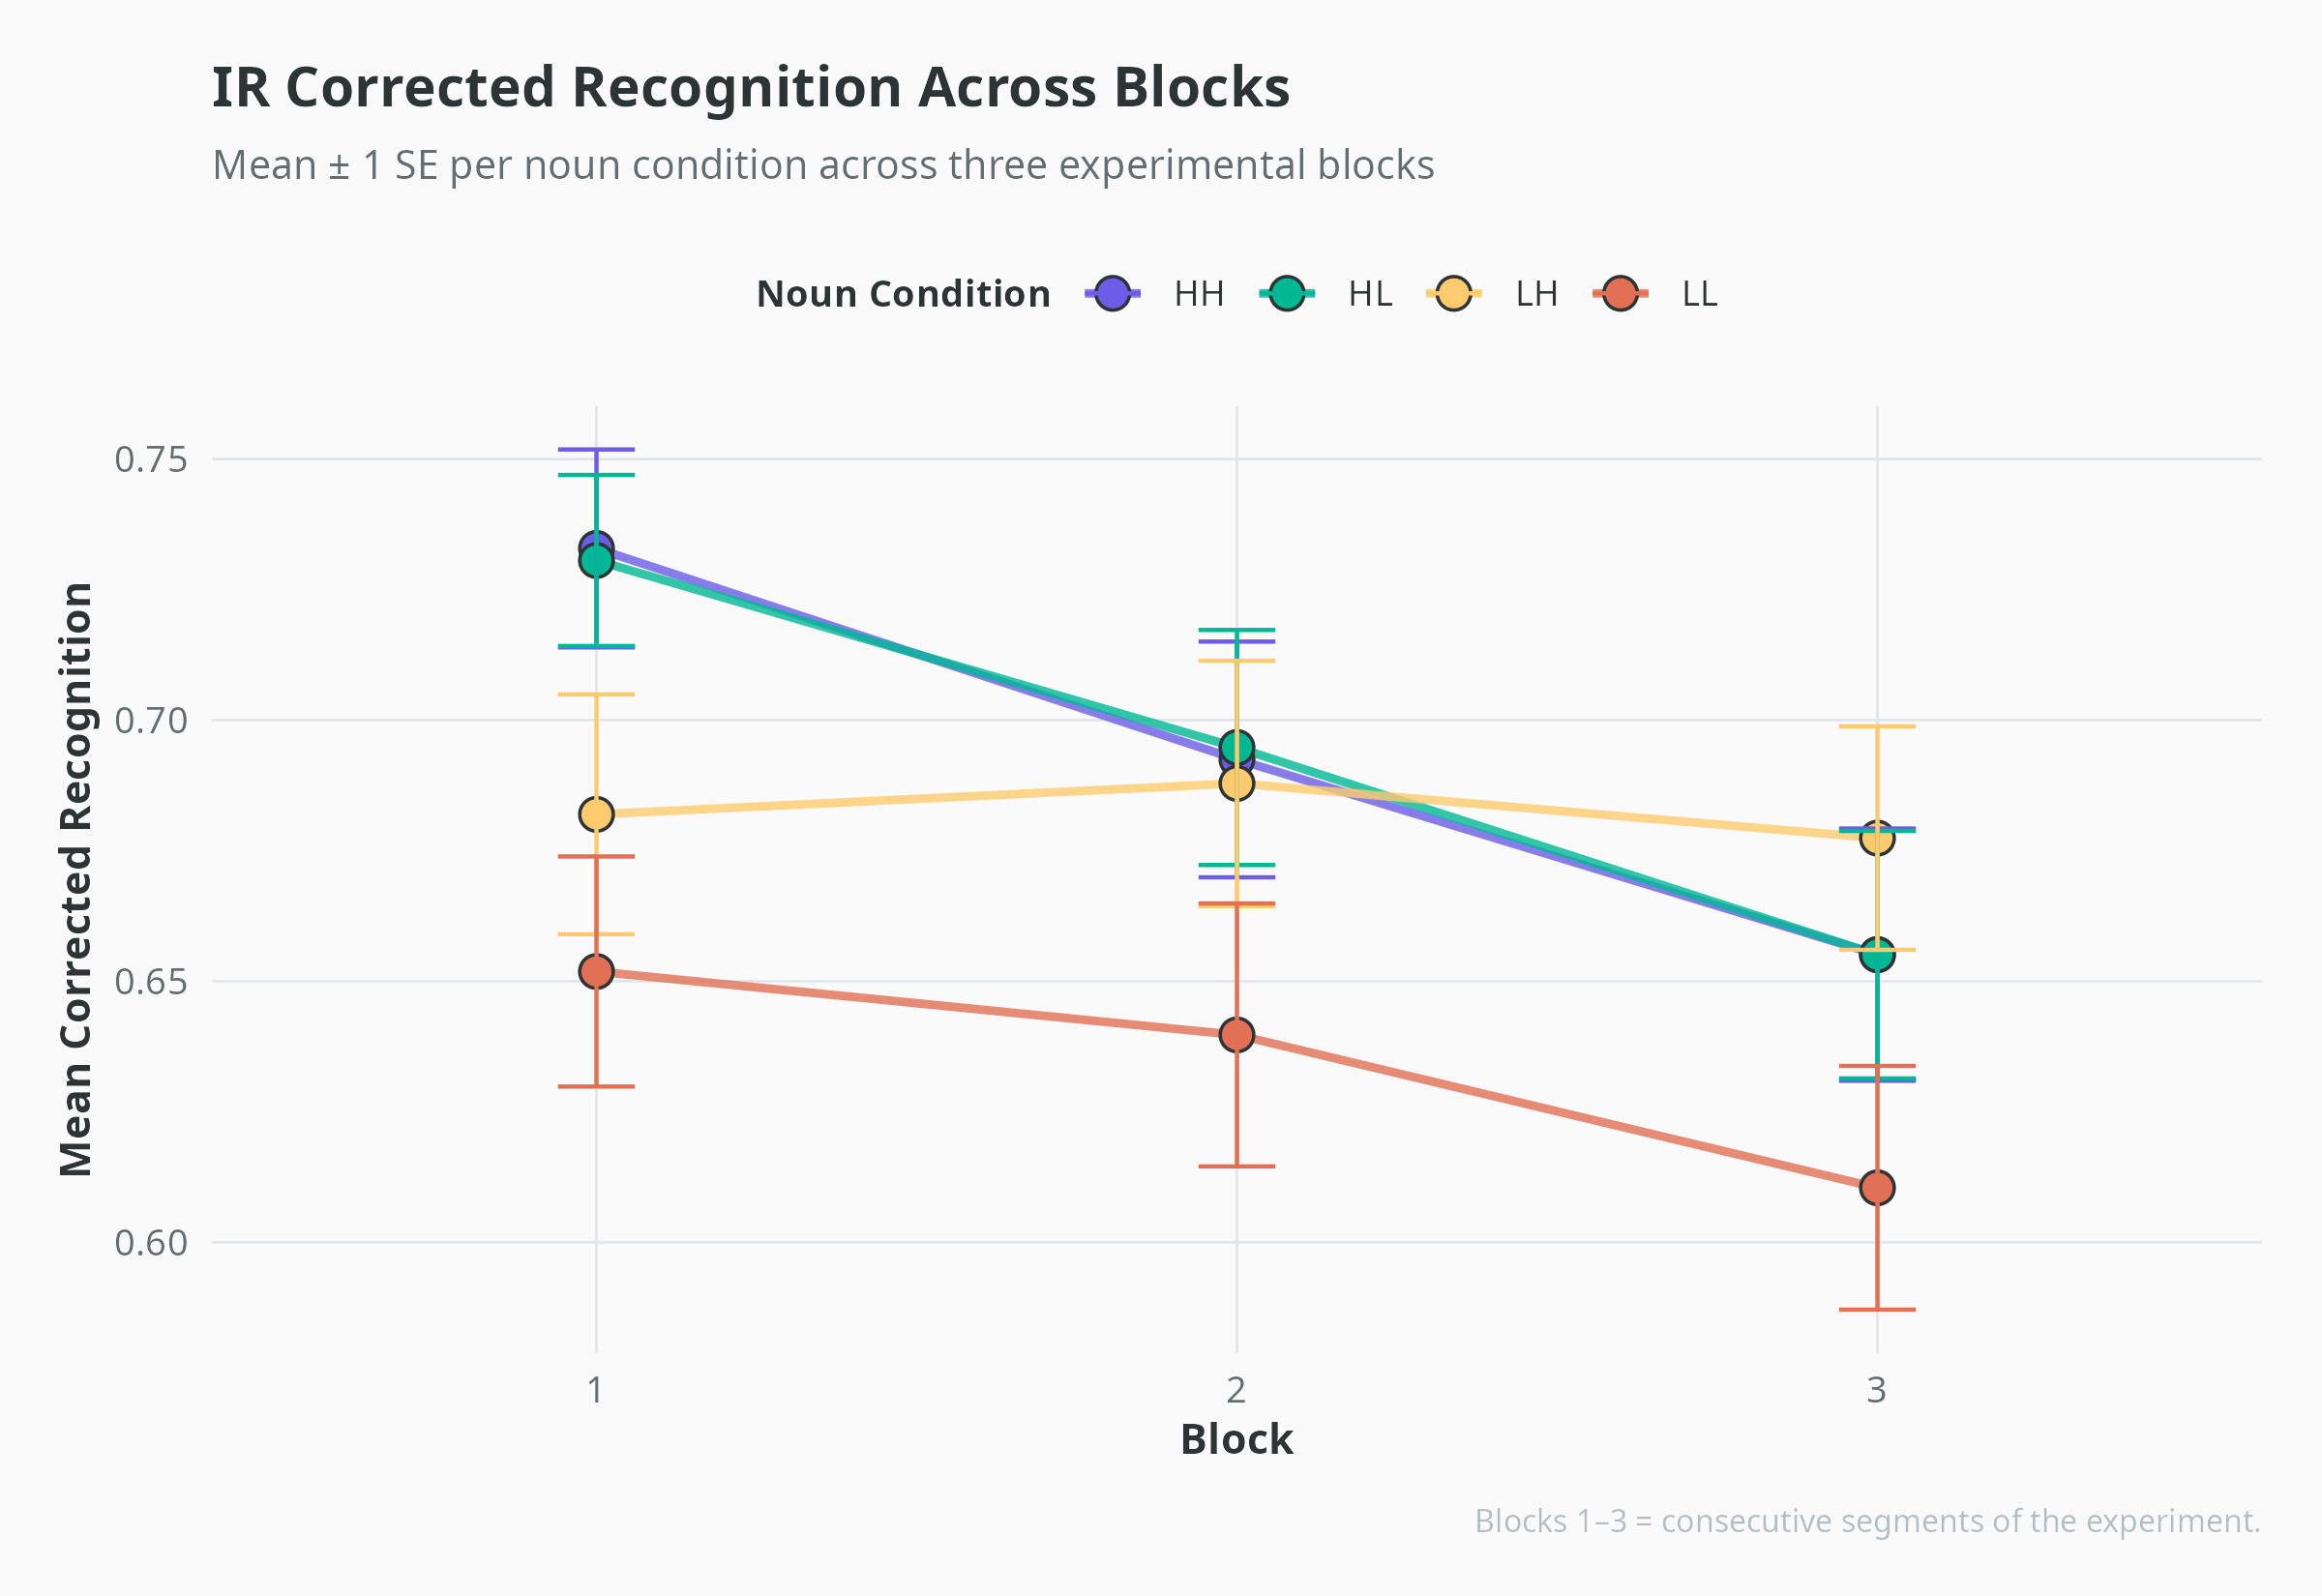
\includegraphics[width=\linewidth]{../../plots/07_block_learning.png}
        \caption{Mean corrected IR ($\pm 1$ SE) by noun condition across
        Blocks 1--3. The downward trend is consistent with mild proactive
        interference but does not reach significance ($H(2) = 2.77$,
        $p = .250$). The LL condition remains consistently below the other
        three throughout.}
        \label{fig:block_learning}
    \end{minipage}\hfill
    \begin{minipage}{0.48\textwidth}
        \centering
        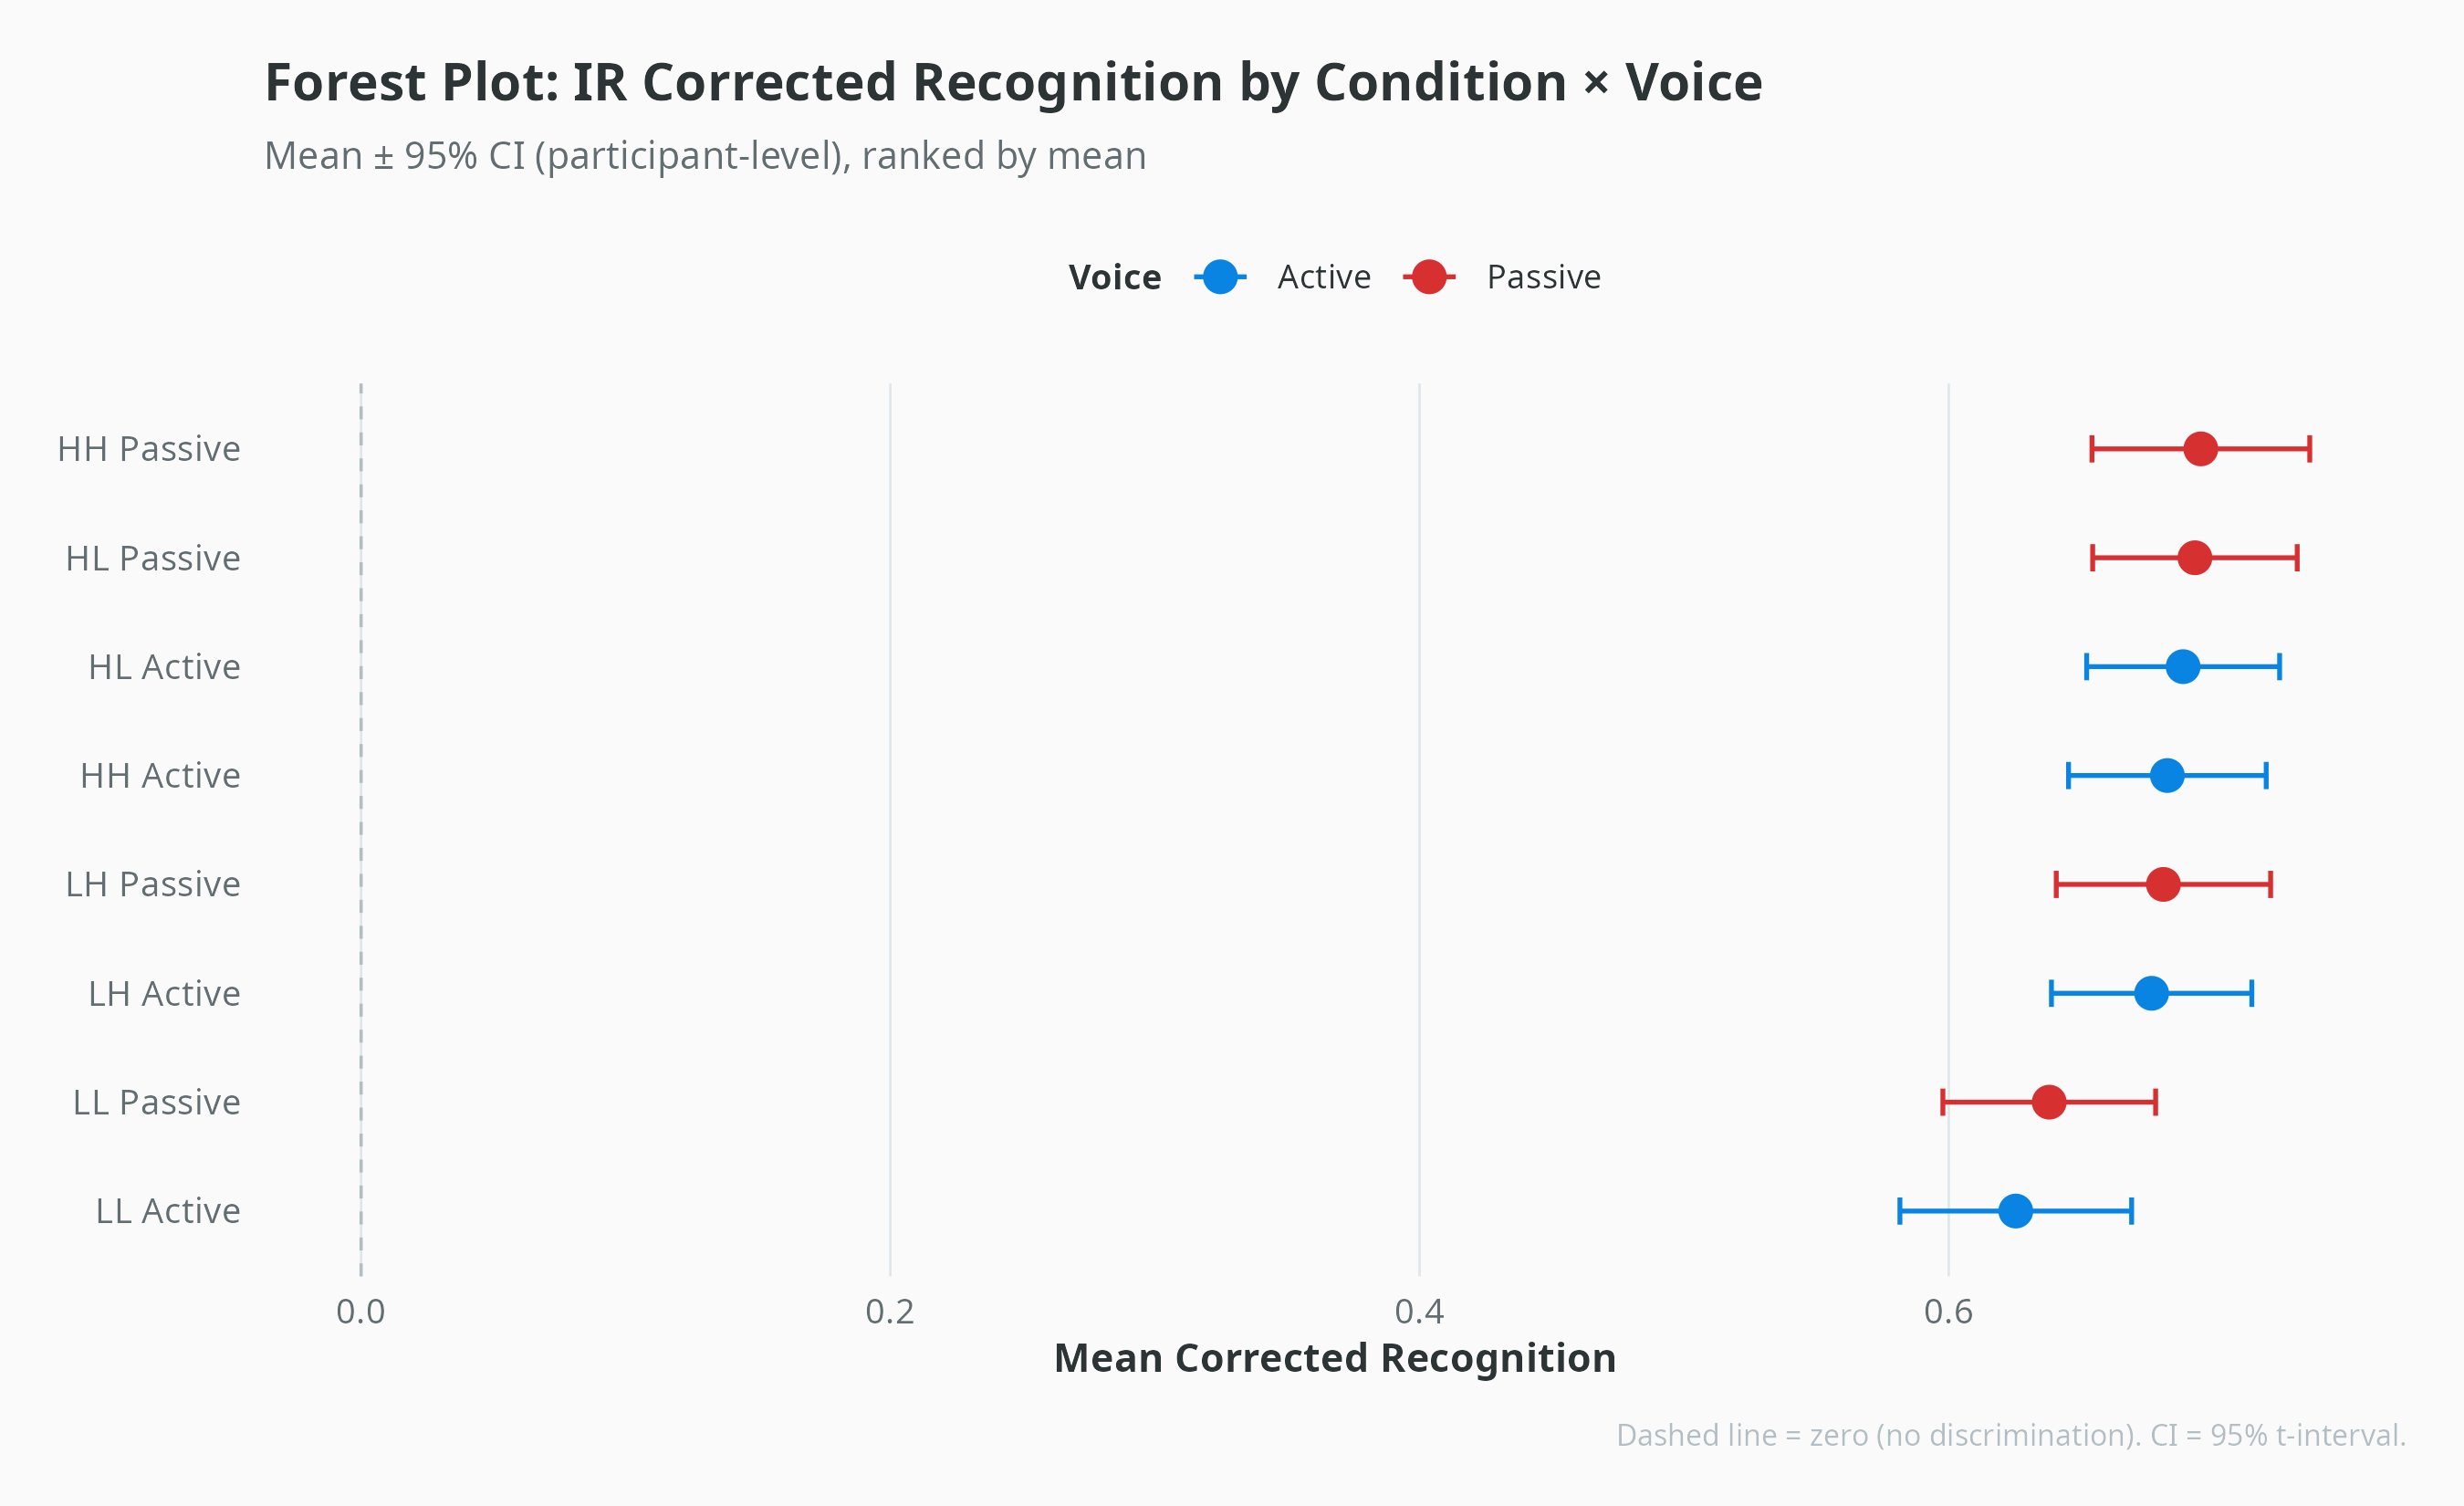
\includegraphics[width=\linewidth]{../../plots/12_forest_plot.png}
        \caption{Forest plot of mean corrected IR ($\pm 95\%$ CI) for all 8
        condition $\times$ voice cells, ranked by mean. The LL conditions
        cluster at the lower end; all 95\% CIs exclude zero, confirming
        above-chance recognition in every cell.}
        \label{fig:forest_plot}
    \end{minipage}
\end{figure}


\subsection{Summary of Statistical Tests}

The forest plot (Figure~\ref{fig:forest_plot}) synthesises all eight
condition $\times$ voice cells. The LL Active and LL Passive conditions cluster
at the lower end; HH, HL, and LH conditions form an elevated cluster between
approximately $M = 0.67$ and $M = 0.70$ with no systematic active--passive
stratification visible, corroborating the null voice effect on IR. All 95\%
confidence intervals exclude zero, confirming above-chance recognition in every
experimental condition. Table~\ref{tab:tests} summarises all primary tests.

\begin{table}[H]
\centering
\caption{Summary of Primary Statistical Tests}
\label{tab:tests}
\begin{tabular}{@{}lcccc@{}}
\toprule
Test & Statistic & $df$ & $p$ & Significant \\ \midrule
KW: IR $\times$ Noun Condition          & $H = 8.85$ & 3  & .031        & Yes \\
KW: WR $\times$ Noun Condition          & $H = 1.98$ & 3  & .576        &     \\
KW: IR $\times$ Block                   & $H = 2.77$ & 2  & .250        &     \\
KW: RT $\times$ Noun Condition          & $H = 4.44$ & 3  & .218        &     \\
WSR: IR Active vs.\ Passive             & $V = 1704$ & -- & .374        &     \\
WSR: WR Active vs.\ Passive             & $V = 3279$ & -- & .113        &     \\
WR vs.\ chance --- Active (one-sample)  & $V = 6322$ & -- & $< .001$    & Yes \\
WR vs.\ chance --- Passive (one-sample) & $V = 5990$ & -- & $< .001$    & Yes \\
\bottomrule
\end{tabular}
\end{table}


% ─────────────────────────────────────────────────────────────
\section{Conclusion and Future Directions}
% ─────────────────────────────────────────────────────────────

This preliminary analysis provides clear evidence that noun imageability
influences sentence recognition, consistent with the reconstructive memory
framework advanced by \citet{james1973} and \citet{begg1971}. The significant
Kruskal-Wallis effect ($H(3) = 8.85$, $p = .031$, $\varepsilon^2 = .054$)
confirms that sentences containing only low-imageability nouns (LL) are
recognised less reliably than those containing at least one high-imageability
noun. Critically, this recognition pattern takes a \textit{threshold} form
rather than the graded one documented by \citet{james1973} in free recall,
where HH $>$ HL $\approx$ LH $>$ LL. This divergence is theoretically
meaningful: in recall, each noun's imageability contributed additively to
reconstruction success, whereas in recognition a single high-imageability
noun appears sufficient to generate a retrievable image trace. Whether this
reflects a fundamental difference between recognition and recall, or simply
a task-difficulty ceiling, requires the full planned sample and mixed-effects
modelling to resolve.

Grammatical voice had no detectable influence on IR ($V = 1704$, $p = .374$),
directly replicating \citeauthor{begg1971}'s (\citeyear{begg1971}) finding
that meaning recognition is equally accurate for identical and paraphrase probes.
Wording recognition (WR), while reliably above chance for both active
($V = 6322$, $p < .001$) and passive sentences ($V = 5990$, $p < .001$) —
consistent with \citeauthor{bregman1968}'s (\citeyear{bregman1968}) above-chance
second-guess performance for the active--passive distinction — was also unaffected
by noun imageability ($H(3) = 1.98$, $p = .576$). This double dissociation
confirms that the mechanism supporting voice discrimination is independent of
the semantic encoding strength that drives IR. The modest positive correlation
between IR and WR (Spearman $\rho = .248$, $p < .001$) is consistent with
Begg's (\citeyear{begg1971}) approximately independent but co-varying
dual-trace model.

\textbf{Next Steps for Report 2.} The present sample ($N = 114$) is
substantially below the targeted $N = 334$, limiting statistical power for
detecting interaction effects and precluding parametric modelling. Report 2
will address this through:
\begin{enumerate}
    \item \textbf{Generalised Linear Mixed Models (GLMMs):} Mixed-effects
    logistic regression will model IR accuracy as a function of Noun Condition
    and Voice as fixed effects, with random intercepts and slopes for both
    Participant and Item. This framework accounts for by-participant and
    by-item variability simultaneously, substantially increasing power
    relative to the participant-aggregated non-parametric tests used here.
    \item \textbf{Reaction Time Modelling:} Log-transformed RT will be analysed
    with linear mixed models to test whether noun imageability predicts
    recognition speed — a proxy for trace strength — independent of its effect
    on accuracy. A speed advantage for high-imageability conditions would provide
    converging evidence for the image-trace hypothesis of \citet{begg1971}.
    \item \textbf{Confirmatory Power Analysis:} Effect sizes from the present
    preliminary analysis (KW $\varepsilon^2 = .054$) will be used to verify
    that the targeted $N = 334$ provides $\geq 80\%$ power for all primary
    contrasts.
\end{enumerate}

\bibliographystyle{plainnat}
\bibliography{references}

\end{document}
